%%%%%%%%%%%%%%%%%%%%%%%%%%%%%%%%%%%%%%%%
% datoteka diploma-FRI-vzorec.tex
%
% vzorčna datoteka za pisanje diplomskega dela v formatu LaTeX
% na UL Fakulteti za računalništvo in informatiko
%
% na osnovi starejših verzij vkup spravil Franc Solina, maj 2021
% prvo verzijo je leta 2010 pripravil Gašper Fijavž
%
% za upravljanje z literaturo ta vezija uporablja BibLaTeX
%
% svetujemo uporabo Overleaf.com - na tej spletni implementaciji LaTeXa ta vzorec zagotovo pravilno deluje
%

\documentclass[a4paper,12pt,openright]{book}
%\documentclass[a4paper, 12pt, openright, draft]{book}  Nalogo preverite tudi z opcijo draft, ki pokaže, katere vrstice so predolge! Pozor, v draft opciji, se slike ne pokažejo!
 
\usepackage[utf8]{inputenc}   % omogoča uporabo slovenskih črk kodiranih v formatu UTF-8
\usepackage[slovene,english]{babel}    % naloži, med drugim, slovenske delilne vzorce
\usepackage[pdftex]{graphicx}  % omogoča vlaganje slik različnih formatov
\usepackage{fancyhdr}          % poskrbi, na primer, za glave strani
\usepackage{amssymb}           % dodatni matematični simboli
\usepackage{amsmath}           % eqref, npr.
\usepackage{hyperxmp}
\usepackage{mathtools}
\usepackage{todonotes}
\usepackage{subcaption} %  for subfigures environments 
\usepackage{placeins}
\usepackage{diagbox}
\usepackage[hyphens]{url}
\usepackage{csquotes}
\usepackage{float}
\usepackage{amsthm}
\usepackage[pdftex, colorlinks=true,
						citecolor=black, filecolor=black, 
						linkcolor=black, urlcolor=black,
						pdfproducer={LaTeX}, pdfcreator={LaTeX}]{hyperref}

\usepackage{color}
\usepackage{soul}

\usepackage[
backend=biber,
style=numeric,
sorting=nty,
]{biblatex}


\addbibresource{literatura.bib} %Imports bibliography file


%%%%%%%%%%%%%%%%%%%%%%%%%%%%%%%%%%%%%%%%
%	DIPLOMA INFO
%%%%%%%%%%%%%%%%%%%%%%%%%%%%%%%%%%%%%%%%
\newcommand{\ttitle}{Algoritmi za reševanje problema matričnih napolnitev}
\newcommand{\ttitleEn}{Diploma thesis template}
\newcommand{\tsubject}{\ttitle}
\newcommand{\tsubjectEn}{\ttitleEn}
\newcommand{\tauthor}{Matej Klančar}
\newcommand{\tkeywords}{računalnik, računalnik, računalnik}
\newcommand{\tkeywordsEn}{computer, computer, computer}
\newcommand{\nnorm}[1]{\lVert#1\rVert_*}
\newcommand{\fnorm}[1]{\lVert#1\rVert_F}
\newcommand{\norm}[1]{\lVert#1\rVert}
\DeclareMathOperator{\diag}{diag}
\DeclareMathOperator{\tr}{Tr}


%%%%%%%%%%%%%%%%%%%%%%%%%%%%%%%%%%%%%%%%
%	HYPERREF SETUP
%%%%%%%%%%%%%%%%%%%%%%%%%%%%%%%%%%%%%%%%
\hypersetup{pdftitle={\ttitle}}
\hypersetup{pdfsubject=\ttitleEn}
\hypersetup{pdfauthor={\tauthor}}
\hypersetup{pdfkeywords=\tkeywordsEn}

%%%%%%%%%%%%%%%%%%%%%%%%%%%%%%%%%%%%%%%%
% postavitev strani
%%%%%%%%%%%%%%%%%%%%%%%%%%%%%%%%%%%%%%%%  

\addtolength{\marginparwidth}{-20pt} % robovi za tisk
\addtolength{\oddsidemargin}{40pt}
\addtolength{\evensidemargin}{-40pt}

\renewcommand{\baselinestretch}{1.3} % ustrezen razmik med vrsticami
\setlength{\headheight}{15pt}        % potreben prostor na vrhu
\renewcommand{\chaptermark}[1]%
{\markboth{\MakeUppercase{\thechapter.\ #1}}{}} \renewcommand{\sectionmark}[1]%
{\markright{\MakeUppercase{\thesection.\ #1}}} \renewcommand{\headrulewidth}{0.5pt} \renewcommand{\footrulewidth}{0pt}
\fancyhf{}
\fancyhead[LE,RO]{\sl \thepage} 
%\fancyhead[LO]{\sl \rightmark} \fancyhead[RE]{\sl \leftmark}
\fancyhead[RE]{\sc \tauthor}              % dodal Solina
\fancyhead[LO]{\sc Diplomska naloga}     % dodal Solina


\newcommand{\BibLaTeX}{{\sc Bib}\LaTeX}
\newcommand{\BibTeX}{{\sc Bib}\TeX}

%%%%%%%%%%%%%%%%%%%%%%%%%%%%%%%%%%%%%%%%
% naslovi
%%%%%%%%%%%%%%%%%%%%%%%%%%%%%%%%%%%%%%%%  

\newcommand{\autfont}{\Large}
\newcommand{\titfont}{\LARGE\bf}
\newcommand{\clearemptydoublepage}{\newpage{\pagestyle{empty}\cleardoublepage}}
\setcounter{tocdepth}{1}	      % globina kazala

%%%%%%%%%%%%%%%%%%%%%%%%%%%%%%%%%%%%%%%%
% konstrukti
%%%%%%%%%%%%%%%%%%%%%%%%%%%%%%%%%%%%%%%%  
\newtheorem{izrek}{Izrek}[chapter]
\newtheorem{trditev}{Trditev}[izrek]
\newenvironment{dokaz}{\emph{Dokaz.}\ }{\hspace{\fill}{$\Box$}}

\newcommand{\CR}[1]{\begin{color}{red}#1\end{color}}
\newcommand{\CB}[1]{\begin{color}{blue}#1\end{color}}
\newcommand{\CG}[1]{\begin{color}{green}#1\end{color}}

\newcommand{\proj}{\mathcal{P}_\Omega}
\newcommand{\shrink}{\mathcal{D}}
%\newcommand{\tr}{\text{Tr}}
\newcommand{\numberthis}{\addtocounter{equation}{1}\tag{\theequation}}
\newcommand{\trOp}[2]{\langle #1, #2 \rangle}
\newcommand{\mapa}{Poglavja}

\newtheorem{theorem}{Izrek}

%%%%%%%%%%%%%%%%%%%%%%%%%%%%%%%%%%%%%%%%%%%%%%%%%%%%%%%%%%%%%%%%%%%%%%%%%%%%%%%
%% PDF-A
%%%%%%%%%%%%%%%%%%%%%%%%%%%%%%%%%%%%%%%%%%%%%%%%%%%%%%%%%%%%%%%%%%%%%%%%%%%%%%%

%%%%%%%%%%%%%%%%%%%%%%%%%%%%%%%%%%%%%%%% 
% define medatata
%%%%%%%%%%%%%%%%%%%%%%%%%%%%%%%%%%%%%%%% 
\def\Title{\ttitle}
\def\Author{\tauthor, matjaz.kralj@fri.uni-lj.si}
\def\Subject{\ttitleEn}
\def\Keywords{\tkeywordsEn}

%%%%%%%%%%%%%%%%%%%%%%%%%%%%%%%%%%%%%%%% 
% \convertDate converts D:20080419103507+02'00' to 2008-04-19T10:35:07+02:00
%%%%%%%%%%%%%%%%%%%%%%%%%%%%%%%%%%%%%%%% 
\def\convertDate{%
    \getYear
}

{\catcode`\D=12
 \gdef\getYear D:#1#2#3#4{\edef\xYear{#1#2#3#4}\getMonth}
}
\def\getMonth#1#2{\edef\xMonth{#1#2}\getDay}
\def\getDay#1#2{\edef\xDay{#1#2}\getHour}
\def\getHour#1#2{\edef\xHour{#1#2}\getMin}
\def\getMin#1#2{\edef\xMin{#1#2}\getSec}
\def\getSec#1#2{\edef\xSec{#1#2}\getTZh}
\def\getTZh +#1#2{\edef\xTZh{#1#2}\getTZm}
\def\getTZm '#1#2'{%
    \edef\xTZm{#1#2}%
    \edef\convDate{\xYear-\xMonth-\xDay T\xHour:\xMin:\xSec+\xTZh:\xTZm}%
}

%\expandafter\convertDate\pdfcreationdate 

%%%%%%%%%%%%%%%%%%%%%%%%%%%%%%%%%%%%%%%%
% get pdftex version string
%%%%%%%%%%%%%%%%%%%%%%%%%%%%%%%%%%%%%%%% 
\newcount\countA
\countA=\pdftexversion
\advance \countA by -100
\def\pdftexVersionStr{pdfTeX-1.\the\countA.\pdftexrevision}


%%%%%%%%%%%%%%%%%%%%%%%%%%%%%%%%%%%%%%%%
% XMP data
%%%%%%%%%%%%%%%%%%%%%%%%%%%%%%%%%%%%%%%%  
\usepackage{xmpincl}
%\includexmp{pdfa-1b}

%%%%%%%%%%%%%%%%%%%%%%%%%%%%%%%%%%%%%%%%
% pdfInfo
%%%%%%%%%%%%%%%%%%%%%%%%%%%%%%%%%%%%%%%%  
\pdfinfo{%
    /Title    (\ttitle)
    /Author   (\tauthor, damjan@cvetan.si)
    /Subject  (\ttitleEn)
    /Keywords (\tkeywordsEn)
    /ModDate  (\pdfcreationdate)
    /Trapped  /False
}

%%%%%%%%%%%%%%%%%%%%%%%%%%%%%%%%%%%%%%%%
% znaki za copyright stran
%%%%%%%%%%%%%%%%%%%%%%%%%%%%%%%%%%%%%%%%  

\newcommand{\CcImageCc}[1]{%
	
\includegraphics[scale=#1]{cc_cc_30.pdf}%
}
\newcommand{\CcImageBy}[1]{%
	
\includegraphics[scale=#1]{cc_by_30.pdf}%
}
\newcommand{\CcImageSa}[1]{%
	
\includegraphics[scale=#1]{cc_sa_30.pdf}%
}

%%%%%%%%%%%%%%%%%%%%%%%%%%%%%%%%%%%%%%%%%%%%%%%%%%%%%%%%%%%%%%%%%%%%%%%%%%%%%%%
%%%%%%%%%%%%%%%%%%%%%%%%%%%%%%%%%%%%%%%%%%%%%%%%%%%%%%%%%%%%%%%%%%%%%%%%%%%%%%%

\begin{document}
\selectlanguage{slovene}
\frontmatter
\setcounter{page}{1} %
\renewcommand{\thepage}{}       % preprečimo težave s številkami strani v kazalu

%%%%%%%%%%%%%%%%%%%%%%%%%%%%%%%%%%%%%%%%
%naslovnica
\thispagestyle{empty}%
\begin{center}
    {\large\sc Univerza v Ljubljani\\%
        %      Fakulteta za elektrotehniko\\% za študijski program Multimedija
        %      Fakulteta za upravo\\% za študijski program Upravna informatika
        Fakulteta za računalništvo in informatiko\\%
        %      Fakulteta za matematiko in fiziko\\% za študijski program Računalništvo in matematika
    }
    \vskip 10em%
        {\autfont \tauthor\par}%
        {\titfont \ttitle \par}%
        {\vskip 3em \textsc{DIPLOMSKO DELO\\[5mm]         % dodal Solina za ostale študijske programe
                %    VISOKOŠOLSKI STROKOVNI ŠTUDIJSKI PROGRAM\\ PRVE STOPNJE\\ RAČUNALNIŠTVO IN INFORMATIKA}\par}%
                UNIVERZITETNI  ŠTUDIJSKI PROGRAM\\ PRVE STOPNJE\\ RAČUNALNIŠTVO IN INFORMATIKA}\par}%
    %    INTERDISCIPLINARNI UNIVERZITETNI\\ ŠTUDIJSKI PROGRAM PRVE STOPNJE\\ MULTIMEDIJA}\par}%
    %    INTERDISCIPLINARNI UNIVERZITETNI\\ ŠTUDIJSKI PROGRAM PRVE STOPNJE\\ UPRAVNA INFORMATIKA}\par}%
    %    INTERDISCIPLINARNI UNIVERZITETNI\\ ŠTUDIJSKI PROGRAM PRVE STOPNJE\\ RAČUNALNIŠTVO IN MATEMATIKA}\par}%
    \vfill\null%
    % izberite pravi habilitacijski naziv mentorja!
    {\large \textsc{Mentor}: doc.\ dr.\
        Aljaž Zalar\par}%
    {\vskip 2em \large Ljubljana, \the\year \par}%
\end{center}
% prazna stran
%\clearemptydoublepage      
% izjava o licencah itd. se izpiše na hrbtni strani naslovnice

%%%%%%%%%%%%%%%%%%%%%%%%%%%%%%%%%%%%%%%%
%copyright stran
%%%%%%%%%%%%%%%%%%%%%%%%%%%%%%%%%%%%%%%%
\newpage
\thispagestyle{empty}

\vspace*{5cm}
{\small \noindent
    To delo je ponujeno pod licenco \textit{Creative Commons Priznanje avtorstva-Deljenje pod enakimi pogoji 2.5 Slovenija} (ali novej\v so razli\v cico).
    To pomeni, da se tako besedilo, slike, grafi in druge sestavine dela kot tudi rezultati diplomskega dela lahko prosto distribuirajo,
    reproducirajo, uporabljajo, priobčujejo javnosti in predelujejo, pod pogojem, da se jasno in vidno navede avtorja in naslov tega
    dela in da se v primeru spremembe, preoblikovanja ali uporabe tega dela v svojem delu, lahko distribuira predelava le pod
    licenco, ki je enaka tej.
    Podrobnosti licence so dostopne na spletni strani \href{http://creativecommons.si}{creativecommons.si} ali na Inštitutu za
    intelektualno lastnino, Streliška 1, 1000 Ljubljana.

    \vspace*{1cm}
    \begin{center}% 0.66 / 0.89 = 0.741573033707865
        \CcImageCc{0.741573033707865}\hspace*{1ex}\CcImageBy{1}\hspace*{1ex}\CcImageSa{1}%
    \end{center}
}

\vspace*{1cm}
{\small \noindent
    Izvorna koda diplomskega dela, njeni rezultati in v ta namen razvita programska oprema je ponujena pod licenco GNU General Public License,
    različica 3 (ali novejša). To pomeni, da se lahko prosto distribuira in/ali predeluje pod njenimi pogoji.
    Podrobnosti licence so dostopne na spletni strani \url{http://www.gnu.org/licenses/}.
}

\vfill
\begin{center}
    \ \\ \vfill
    {\em
        Besedilo je oblikovano z urejevalnikom besedil \LaTeX.}
\end{center}

% prazna stran
\clearemptydoublepage

%%%%%%%%%%%%%%%%%%%%%%%%%%%%%%%%%%%%%%%%
% stran 3 med uvodnimi listi
\thispagestyle{empty}
\
\vfill

\bigskip
\noindent\textbf{Kandidat:} Matej Klančar\\
\noindent\textbf{Naslov:} Naslov diplomskega dela\\
% vstavite ustrezen naziv študijskega programa!
\noindent\textbf{Vrsta naloge:} Diplomska naloga na univerzitetnem programu prve stopnje Računalništvo in informatika \\
% izberite pravi habilitacijski naziv mentorja!
\noindent\textbf{Mentor:} doc.\ dr.\ Aljaž Zalar\\

\bigskip
\noindent\textbf{Opis:}\\
Besedilo teme diplomskega dela študent prepiše iz študijskega informacijskega sistema, kamor ga je vnesel mentor.
V nekaj stavkih bo opisal, kaj pričakuje od kandidatovega diplomskega dela.
Kaj so cilji, kakšne metode naj uporabi, morda bo zapisal tudi ključno literaturo.

\bigskip
\noindent\textbf{Title:} Algorithms for solving matrix completion problem

\bigskip
\noindent\textbf{Description:}\\
opis diplome v angleščini

\vfill



\vspace{2cm}

% prazna stran
\clearemptydoublepage

% zahvala
\thispagestyle{empty}\mbox{}\vfill\null\it%
\noindent
Na tem mestu zapišite, komu se zahvaljujete za pomoč pri izdelavi diplomske naloge oziroma pri vašem študiju nasploh. Pazite, da ne boste koga pozabili. Utegnil vam bo zameriti. Temu se da izogniti tako, da celotno zahvalo izpustite.
\rm\normalfont

% prazna stran
\clearemptydoublepage

%%%%%%%%%%%%%%%%%%%%%%%%%%%%%%%%%%%%%%%%
% % posvetilo, če sama zahvala ne zadošča :-)
% \thispagestyle{empty}\mbox{}{\vskip0.20\textheight}\mbox{}\hfill\begin{minipage}{0.55\textwidth}%
%     Svoji dragi Alenčici.
%     \normalfont\end{minipage}

% prazna stran
\clearemptydoublepage


%%%%%%%%%%%%%%%%%%%%%%%%%%%%%%%%%%%%%%%%
% kazalo
\pagestyle{empty}
\def\thepage{}% preprečimo težave s številkami strani v kazalu
\tableofcontents{}


% prazna stran
\clearemptydoublepage

%%%%%%%%%%%%%%%%%%%%%%%%%%%%%%%%%%%%%%%%
% seznam kratic

\chapter*{Seznam uporabljenih kratic}

\noindent\begin{tabular}{p{0.11\textwidth}|p{.39\textwidth}|p{.39\textwidth}}    % po potrebi razširi prvo kolono tabele na račun drugih dveh!
    {\bf kratica} & {\bf angleško}                      & {\bf slovensko}                        \\ \hline
    {\bf SVT }    & Singular Value Thresholding         & Prag singularnih vrednosti             \\
    {\bf NNM}     & Nuclear norm minimization           & Minimizacija nuklearne norme           \\
    {\bf TNNM}    & Truncated nuclear norm minimization & Minimizacija prirezane nuklearne norme \\
    {\bf ASD}     & Alternating Steepest Descent        & Izmenjajoč gradientni spust            \\
    {\bf NP}     & Nondeterministic polynomial time       & Nedeterministični polinomni čas            \\
    {\bf SDP}     & Semidefinite programming        & Semidefinitno programiranje            \\
    \CG{\bf OZP}     &         & \CG{Odstotek znanih podatkov}            \\
    %  \dots & \dots & \dots \\
\end{tabular}


% prazna stran
\clearemptydoublepage

%%%%%%%%%%%%%%%%%%%%%%%%%%%%%%%%%%%%%%%%
% povzetek
\phantomsection
\addcontentsline{toc}{chapter}{Povzetek}
\chapter*{Povzetek}

\noindent\textbf{Naslov:} \ttitle
\bigskip

\noindent\textbf{Avtor:} \tauthor
\bigskip

%\noindent\textbf{Povzetek:} 
\noindent V vzorcu je predstavljen postopek priprave diplomskega dela z uporabo okolja \LaTeX. Vaš povzetek mora sicer vsebovati približno 100 besed, ta tukaj je odločno prekratek.
Dober povzetek vključuje: (1) kratek opis obravnavanega problema, (2) kratek opis vašega pristopa za reševanje tega problema in (3) (najbolj uspešen) rezultat ali prispevek diplomske naloge.

\bigskip

\noindent\textbf{Ključne besede:} \tkeywords.
% prazna stran
\clearemptydoublepage

%%%%%%%%%%%%%%%%%%%%%%%%%%%%%%%%%%%%%%%%
% abstract
\phantomsection
\selectlanguage{english}
\addcontentsline{toc}{chapter}{Abstract}
\chapter*{Abstract}

\noindent\textbf{Title:} \ttitleEn
\bigskip

\noindent\textbf{Author:} \tauthor
\bigskip

%\noindent\textbf{Abstract:} 
\noindent This sample document presents an approach to typesetting your BSc thesis using \LaTeX.
A proper abstract should contain around 100 words which makes this one way too short.
\bigskip

\noindent\textbf{Keywords:} \tkeywordsEn.
\selectlanguage{slovene}
% prazna stran
\clearemptydoublepage

%%%%%%%%%%%%%%%%%%%%%%%%%%%%%%%%%%%%%%%%
\mainmatter
\setcounter{page}{1}
\pagestyle{fancy}


% Optional TOC
% \tableofcontents
% \pagebreak
\chapter{Uvod}
\todo{spisi in popravi vse}
\section{Motivacija}
Problem matričnih napolnitev sprejme matriko, največkat označeno z $M$, pri kateri so nekateri elementi označeni kot neznani. Problem nato sprašuje po vrednostih, ki jih lahko vstavimo v neznane vrednosti, tako da bo rang matrike najmanjši možen. Gre za NP-poln problem, zato ga poskušamo poenostaviti, ter reševati lažje probleme, ki vrnejo dovolj dobre, a ne optimalne rešitve. 

Problem je v zadnjih letih zelo popularen, z njim pa se ukvarjajo tako številni matematiki kot računalničarji. Njegova splošnost naredi reševanje problema na številnih področjih, sam pa se v diplomski nalogi osredotočim na razreševanje neznanih pikslov v slikah. Prav tako omenjam in preizkusim algoritem na priporočilnih sistemih. Rezultate teh predstavim v poglavju X.

V tej diplomski nalogi bom predstavil par  algoritmov, ki rešujejo omenjen problem. Algoritmi so bili izbrani glede na njihovo popularnost in priznanost v literaturi. Prav tako sem poskrbel, da so algoritmi primerno različni in temeljijo na drugačnih principih. Algoritme sem tudi implementiral, nato pa še napravil analizo ter opisal ugotovitve v poglavju X.

\section{Cilji}

Nekaj o tem, kaj želimo narediti.

Glavni prispevki tega diplomskega dela so ...

\section{Struktura diplomskega dela}

V poglavju 2 ,,,, v poglavju 3 ....
\chapter{Pregled področja} \label{1407-1010}

Raziskovanje problema matričnih napolnitev (PMN) je zelo aktivno področje, saj se pojavljajo številni članki z novimi pristopi in izboljšavami obstoječih metod.  Splošnost problema in številne uporabe pojasnjujejo motivacijo za iskanje še učinkovitejših oz.\ bolj ciljno usmerjenih algoritmov od obstoječih.

Eno prvih del, ki obravnava PMN, je \cite{MCPAS}. Delo opiše problem in njegovo naravo, poleg napolnitev minimalnega ranga pa obravnava tudi nekatere druge vrste napolnitev. Obravnavane so tudi metode za napolnjevanje matrik s ciljem pozitivne semidefinitnosti napolnitve ali pa s ciljem maksimizacije determinante. Oba problema sta bila obsežno študirana v zadnjih dveh desetletjih 20.\ stoletja \cite{Barret, Dancis,Woerdeman}.

Delo \cite{NNM-PHD} pretvori problem minimizacije ranga napolnitve v problem iz področja semidefinitnega programiranja. Ideje in dokazi tega dela služijo kot temelj za več algoritmov, ki so se razvili v zadnjih letih.
Članek \cite{CCS} opisuje algoritem SVT, katerega ideja temelji na uvedbi \textit{operatorja praga}, ki vse singularne vrednosti manjše od izbranega praga postavi na 0. Članek tudi pokaže, zakaj je tak način reševanja smiselen.
Članek \cite{TNNM-HZYLH12} opisuje algoritem TNNM, ki uporabi informacijo o rangu nezašumljene matrike, in problem rešuje s pomočjo znanega algoritma ADMM \cite{admmForNNM} iz področja reševanja problema vezanih ekstremov. 
Vir \cite{AST-TK15} opisuje algoritem ASD, ki išče matriki $X$ in $Y$, katerih produkt bo enak napolnjeni matriki. Matriki išče z uporabo gradientnega spusta in izračunom optimalnega koraka v smeri gradienta v vsaki iteraciji.  
Algoritem LMaFit, predstavljen v \cite{LMaFit-WY12}, prav tako išče najboljši produkt dveh matrik, vendar pa za iskanje uporablja Moore-Penroseov inverz, ki v vsaki iteraciji najde optimalen rezultat po metodi najmanjših kvadratov.
Obstajajo še številne druge metode, ki temeljijo na drugačnih idejah (npr.\ \cite{admira,Riemannian,SETalgo}), in jih zaradi obsežnosti v tem diplomskem delu ne bomo obravnavali. 


Temeljna literatura pri nastajanju diplomske naloge je bil pregledni članek \cite{Survey-NKS19}, ki opiše problem in v grobem predstavi več algoritmov ter jih primerja. Sicer večina opisov ni dovolj podrobnih, da bi lahko algoritme implementirali, vseeno pa je  članek dobra osnova, saj na kratko poda pregled literature iz področja PMN in ustrezne reference. V članku so algoritmi tudi testirani na izbranem problemu uporabe,
rezultati pa primerjani med seboj. Ravno ta primerjava pa je v večini drugih virih bolj skopo obravnavana.

Kot smo videli zgoraj, obstajajo številni članki s področja PMN. Večina člankov predstavi neko novo metodo, razloži idejo v ozadju, izpelje nekaj konvergenčnih rezultatov in testiranj na izbranem problemu.
Zelo malo pa je literature, ki različne metode primerja med seboj in poskuša klasificirati algoritme glede na to, za kateri problem so najprimernejši. Prav tako je navadno pomanjkljivo razloženo, zakaj je bilo testiranje narejeno ravno na podatkih določenega tipa . Ponekod gre za naključno generirane podatke iz točno določene porazdelitve s točno določeno strukturo, pri čemer od tod ni moč sklepati, kako bi se algoritem obnesel na nekoliko drugačnih podatkih, ki ne bi bili pridobljeni ravno na tovrsten način. V delu se zato želimo osredotočiti tudi na ta vidik, tj.\ na implementacijo algoritmov in testiranje na podatkih istega tipa.

\chapter{Algoritmi}

\CB{Na koncu napisati kratek odstavek o tem, kaj je vsebina poglavja.}

\section{Pomembe definicije}
Nekatere definicije so uporabljene čez več algoritmov. Z namenom preglednosti, te opisujem v tem poglavju
\begin{enumerate}
  \item $\Omega$ je definirana množica znanih vrednosti
  \item \[ [\proj]_{i,j} = \begin{cases}
            a_{ij} & (i, j) \in \Omega \\
            0      & \textrm{drugače}
          \end{cases}
        \]
  \item Operator $\shrink_\tau$ kot \[
            \shrink_\tau(A) := U \shrink_\tau(\Sigma) V^T, \hspace{0.3cm} \shrink_\tau(\Sigma) = diag(max(\sigma_i - \tau, 0))
        \] \cite{CCS}
  \item Z oznako $M \in \mathbb{R}^{n_1 \times n_2}$ označujemo vhodno matriko, torej tisto, ki ima nekatere podatke neznane.
  % \item Z oznako $M \in \mathbb{R}^{n_1 \times n_2}$ označujemo bitno matriko M, ki predstavlja masko, s katero označimo katere vrednosti poznamo in katere ne. Vrednost 1 označuje, da je vrednost na tisti poziciji znana, medtem ko 0 označuje, da ni. 
\end{enumerate}

\section{Minimizacija nuklearne norme}
Ker je minimizacija ranga matrike NP-poln problem, so se razvile druge metode, ki samo kompleksnost problema zmanjšujejo. Minimizacija nuklearne norme (Nuclear Norm Minimization) se zanaša na dejstvo, da je rang matrike povezan z nuklearno normo matrike. Ta je definirana kot
\[
  ||X||_* = \sum_{i = i}^{n} \sigma_i(X)
\] \todo{se lahko sklicujem?}
Dokazano je bilo, da nuklearna norma predstavlja konveksno ovojnico ranga. \cite{NNM-PHD} Konveksna ovojnica funkcije $f : \mathcal{C} \rightarrow \mathbb{R}$ je največja konveksna funkcija $g$ tako da velja $f(x) \geq g(x)$ za vse $x \in \mathcal{C}$. \cite{Survey-NKS19}

Minimizacijo nuklearne norme je možno pretvoriti v semidefinitni problem, ki ga lahko rešujemo z različnimi pripomočki, na primer SeDuMi \cite{SeDuMi}.

Standardna oblika semidefinitnega programa je
\begin{align*}
    \min_Y \hspace{0.5cm} &\trOp{C}{Y} \\
    \text{tako da} \hspace{0.5cm} &\trOp{A_k}{Y} = b_k, \hspace{0.5cm} k = 1, \hdots , l\\
    &Y \succeq 0
\end{align*}
Kjer je $C$ dana matrika, $\{A_k\}$ in $\{b_k\}$ pa množici matrik in vektorjev. 

Problem minimizacije nuklearne norme lahko zapišemo kot 
\begin{align*}
    \min_{X, t} \hspace{0.5cm} &t \\
    \text{tako da} \hspace{0.5cm} &||X||_* \leq t,\\
    &\proj(X) = \proj(M)
\end{align*}
Trdimo, da za matriko $X \in \mathbb{R}^{n_1 \times n_2}$ in $t \in \mathbb{R}$ 
velja $||X||_* \leq t \iff \exists W_1\in \mathbb{R}^{n_1 \times n_1}, W_2 \in \mathbb{R}^{n_2 \times n_2}$ tako da \cite{NNM-PHD} \todo{se lahko sklicujem?}
\begin{align*}
    &Y = \begin{bmatrix}
        W_1 & X \\
        X^T & W_2
    \end{bmatrix}, \\
    &Y \succeq 0, \hspace{0.2cm} \tr(Y) \leq 2t
\end{align*} 

Minimizacijski problem lahko tako redefiniramo kot 
\begin{align*}
    \min_{Y,t} \hspace{0.5cm} &2t\\
    \text{tako da} \hspace{0.5cm} & Y \succeq 0,\\
    &\trOp{Y}{A_{a,b}} = b_{a,b}
\end{align*} 
kjer je $A_{a,b} \in \mathbb{R}^{(n_1 + n_2) \times (n_1 + n_2)}$ matrika v množici $A$. Velja 
$A_{a, b} \in A \iff (a, b) \in \Omega$. Matrika $A_{a,b}$ ima vse elemente ničelne, razen na mestu $(a, n_1 + b)$, kjer ima vrednost $1$.
Podobno je definiran tudi $b_{a,b} \in \mathbb{R}$, ki ima vrednost $M_{a, b}$.
Ker velja 
\[
    \trOp{A}{B} = \sum_{i}^{n_1} \sum_{j}^{n_2} a_{i,j}b_{i,j}
\] je lahko videti, da je tak pogoj smiselen. Programi za reševanje SDP pa lahko tako obliko že sprejmejo.
\cite{Survey-NKS19}


% Za SVD razcep matrike $X = U\Sigma V^T$ velja 
% \[
%     \tr \begin{bmatrix}
%         UU^T & -UV^T \\
%         -VU^T & VV^T
%     \end{bmatrix}
%     \begin{bmatrix}
%         Y & X \\
%         X^T & Z
%     \end{bmatrix} \geq 0
% \] \todo{zakaj je prva matrika pozitivno semidefinitna?}
% ker je vsota diagonalnih elementov produkta dveh pozitivnih semidefinitnih matrik vedno nenegativna. Tako vemo, da 
% \[
%     \tr(UU^TY) - \tr(UV^TX^T) - \tr(VU^TX) + \tr(VV^TZ) \geq 0
% \]

% Po \cite{CR08} lahko problem definiramo kot
% \begin{align*}
%   \min    & \hspace{0.5cm} \tr(Y)                                    \\
%   \text{tako da} & \hspace{0.5cm} (Y, A_k) = b_k, k = 1, \cdots , |\Omega| \\
%                     & \hspace{0.5cm} Y \succcurlyeq 0
% \end{align*}
% kjer
% \begin{align*}
%   &Y = \begin{bmatrix}
%     W_1 & X   \\
%     X^T & W_2
%   \end{bmatrix}
% \end{align*} tak problem pa lahko že rešujemo s semidefinitnimi programi.
\section{Algoritem praga singularnih vrednosti}\label{2807-1441}
\textbf{Algoritem praga singularnih vrednosti (SVT)} \cite{CCS} uporabi idejo, da imajo matrike z majhnim rangom nekaj velikih singularnih vrednosti, ostale pa 0 ali pa vsaj blizu 0. Ključna parametra v SVT-ju sta \textit{izbira premika} in \textit{izbira praga},  
%Za svoje delovanje uvede dva nova pomembna koncepta, prvi je premik, drugi pa prag, potreben za uporabo operatorja $\shrink_\tau$ \eqref{1007-1959}. 
algoritem pa temelji na iteraciji
\begin{align}
\label{2407-1910}
        X^{(k)} &= \shrink_\tau(Y^{(k-1)}), \\
        Y^{(k)} &= Y^{(k-1)} + \delta_k \proj(M - X^{(k)}), 
\end{align}
kjer so $\tau > 0$ izbran prag, $\delta_k$ izbran premik, $X^{(0)} = 0 \in \mathbb{R}^{n_1 \times n_2}$ in
$Y^{(0)} = 0 \in \mathbb{R}^{n_1 \times n_2}$. \cite{CCS}

V nadaljevanju bomo opisali glavno idejo zgornje iteracije. V grobem pa temelji na uporabi metode za iskanje vezanih ekstremov, kjer elementi matrik $Y^{(k)}$ predstavljajo Lagrangove množitelje. 

Uvedimo funkcijo 
\begin{align}
    \label{1007-2007}
    f_\tau(X) = \tau\nnorm{X} + \frac{1}{2}\fnorm{X}^2
\end{align}
in optimizacijski problem
\begin{align}
\label{2706-0957}
\begin{split}
    \min_{X\in \mathbb R^{n_1\times n_2}} & \hspace{0.5cm} f_\tau(X), \\
    \textrm{pri pogojih} & \hspace{0.5cm} \proj(X) = \proj(M).
\end{split}
\end{align}
Opazimo lahko, da za velike vrednosti $\tau$ velja $f_\tau(X) \approx \tau\nnorm{X}$, kar pomeni, da bo s primerno izbranim $\tau$, optimizacijski problem minimiziral nuklearno normo.

Denimo, da želimo poiskati minimum funkcije $f(x)$ pri pogojih $g_1(x)=g_2(x)=\ldots=g_{k}(x)=0$.
V teoriji vezanih ekstremov se za tovrstne probleme uvede \textbf{Lagrangeovo funkcijo}
\[\mathcal{L}(x, \lambda_1,\lambda_2,\ldots,\lambda_k) = f(x) + \lambda_1 g_1(x)+\lambda_2g_2(x)+\ldots+\lambda_kg_k(x),\]
nato pa išče ekstreme med njenimi stacionarnimi točkami.
Problemu \eqref{2706-0957} lahko priredimo Lagrangeovo funkcijo
\[
    \mathcal{L}(X, Y) = f_\tau(X) + \left< Y, \proj(M - X) \right>,
\] 
nato pa iščemo njene stacionarne točke.
Zaradi velikega števila parametrov pa ta pristop navadno ni izvedljiv, zato se v SVT-ju za iskanje ekstremov $\mathcal{L}(X, Y)$ uporabi t.i.\ \textit{Uzawa algoritem} \cite{CCS}. Ta ekstreme išče prek iterativnega postopka:
\begin{align}
        X^{(k)} &=  \argmin_{X} \mathcal{L}(X^{(k)}, Y^{(k-1)}) \label{1007-2018},\\
        Y^{(k)} &= Y^{(k-1)} + \delta_k \proj(M - X^{(k)}). \label{1007-2019}
\end{align}

Izkaže se, da je rešitev \eqref{1007-2018} enaka $\shrink_\tau(Y^{(k-1)})$. To spodaj dokažemo, še prej pa izpeljimo pomožen rezultat.

\begin{trditev}
Velja:
\begin{align}
    \argmin_X  \mathcal{L}(X, Y)
    = \argmin_X \Big(\tau\nnorm{X} + \frac{1}{2}\fnorm{X - Y}^2\Big)
\end{align}
\end{trditev}

\begin{proof}
Trditev sledi iz krajšega računa:
\begin{align*}
    &\argmin_X  \Big(\tau\nnorm{X} + \frac{1}{2}\fnorm{X - Y}^2\Big) \\
    &=\argmin_X \Big(\tau\nnorm{X} + \frac{1}{2}\trOp{X - Y}{X - Y}\Big)\\
    &=\argmin_X \Big(\tau\nnorm{X} + \frac{1}{2}(\fnorm{X}^2 - 2\trOp{X}{Y} + \fnorm{Y}^2)\Big) \\ 
    &=\argmin_X \Big(\tau\nnorm{X} + \frac{1}{2}\fnorm{X}^2 - \trOp{X} {\proj(Y)}\Big)\\
    &=\argmin_X \Big(\tau\nnorm{X} + \frac{1}{2}\fnorm{X}^2 + \tr(- \proj(X)Y^T) + \tr(\proj(M)Y^T)\Big)\\
    &=\argmin_X \Big(\tau\nnorm{X} + \frac{1}{2}\fnorm{X}^2 + \tr(\proj(M - X)Y^T)\Big)\\
    &=\argmin_X \Big(\tau\nnorm{X} + \frac{1}{2}\fnorm{X}^2 + \trOp{Y}{\proj(M - X)}\Big)\\ 
    &= \argmin_X \mathcal{L}(X, Y)
\end{align*}
kjer smo v prvi enakosti uporabili definicijo Frobeniusove norme, v drugi bilinearnost skalarnega produkta, 
v tretji smo ignorirali konstanto $\fnorm{Y}^2$, saj ne vpliva na rezultat, 
in upoštevali $\proj(Y^{(k)}) = Y^{(k)}$ za vse $k \in \mathbb{N}$. Zadnje dejstvo sledi iz definicije \eqref{1007-2019} in $Y^{(0)} = 0$. V četrti enakosti smo upoštevali $\trOp{X}{\proj(Y)} = \trOp{\proj(X)}{Y}$, kar je lahko videti, ko se spomnimo, da za skalarni produkt $\trOp{A}{B}$ matrik $A, B \in \mathbb{R}^{n_1 \times n_2}$ velja 
\[
    \trOp{A}{B} = \sum_{i = 1}^{n_1}\sum_{j = 1}^{n_2} a_{ij}b_{ij}.
\]
Prišteli smo tudi konstanto $\tr(\proj(M)Y^T)$, ki ne vpliva na rezultat.
V peti enakosti smo upoštevali linearnost sledi in aditivnost operatorja $P_\Omega$,
v šesti definicijo skalarnega produkta in v zadnji definicijo Lagrangeove funkcije.
\end{proof}
\begin{theorem} \label{1907-2240}
Za matriki $X \in \mathbb{R}^{n_1 \times n_2}$ in 
$Y \in \mathbb{R}^{n_1 \times n_2}$ velja:
\begin{align}
    \label{2906-1056}
    \shrink_\tau(Y) = \argmin_{X} \Big(\frac{1}{2} \fnorm{X-Y}^2 + \tau\nnorm{X} \Big) 
\end{align}
\end{theorem}

\begin{proof} 
Najprej se spomnimo definicije konveksne funkcije. Funkcija $f$ je konveksna, če za katerikoli dve točki $x_1, x_2$ v domeni funkcije $f$ velja, da je premica čez ti dve točki na odseku med tema dvema točkama nad grafom funkcije $f$.
Funkcija $h(X) := \frac{1}{2} \fnorm{X-Y}^2 + \tau\nnorm{X} $ je konveksna funkcija, saj potreben pogoj trikotniške neenakosti matričnih norm zagotavlja, da je matrična norma konveksna funkcija. Vsota konveksnih funkcij pa je prav tako konveksna funkcija. 
%\todo{ali je potrebno citirati} 
Zaradi konveksnosti funkcije $f$ je 
subgradient v vsaki točki iz domene dobro definiran.
Tega smo definirali v razdelku \ref{2607-1502}.
Matrika $Z\in \mathbb R^{n_1\times n_2}$ je subgradient funkcije $f$ v točki 
$X_0\in \mathbb R^{n_1\times n_2}$,
če velja 
\[\forall X\in \mathbb R^{n_1\times n_2}: 
f(X) \geq  f(X_0) + \trOp{Z}{X - X_0}.\]
Iz definicije subgradienta sledi, da bo imela funkcija $f$ minimum v točki $X'$ natanko tedaj,
ko bo ničelna matrika $\mathbf{0}$ eden izmed subgradientov funkcije $f$ v točki $X_0$.
\iffalse 
V minimumu funkcije $f$ bo eden od subgradientov iščemo minimum $X'$ funkcije $f$,  iščemo tako točko $X'$, da bo
\CG{eden izmed subgradientov po spremenljivki $X$} v točki $X'$ enak 0.  
\fi 

Izkaže se \cite{CCS}, da je množica subgradientov nuklearne norme v točki $X$ enaka
\begin{equation}  \label{2807-0932}  
    \partial\nnorm{X} = \{UV^* + W: W \in \mathbb{R}^{n_1 \times n_2}, U^*W = \mathbf{0}, WV = \mathbf{0}, \norm{W}_2 \leq 1 \},
\end{equation}
kjer $U \Sigma V^T$ predstavlja SVD razcep matrike $X$. S krajšim računom lahko preverimo, da za vsak par $(i,j)$ velja $\frac{\partial}{\partial X_{ij}}\fnorm{X-Y}^2 = 2(X_{ij} - Y_{ij})$. 
Če te parcialne odvode zložimo v matriko, dobimo $2(X-Y)$. Od tod sledi, da je $X-Y$ eden od subgradientov funkcije $h_1(X):=\frac{1}{2}\fnorm{X-Y}^2$ v točki $X$ \cite[3.1.3]{boyd2004convex}.
Iz teh dveh premislekov sledi, da bo $X'$ minimum $h$ natanko tedaj, ko velja 
\begin{equation} \label{2807-0940}
    \mathbf{0} \in X' - Y + \tau \partial\nnorm{X'}.
\end{equation}
Trditev izreka bo sledila, če pokažemo, da velja $X' = \shrink_\tau(Y)$. Najprej razčlenimo SVD razcep matrike $Y$ kot 
\[
    Y = U_0\Sigma_0V_0^T + U_1\Sigma_1V_1^T,
\]
kjer se $U_0, \Sigma_0$ in $V_0$ nanaša na singularne vrednosti in pripadajoče singularne vektorje večje od $\tau$, $U_1, \Sigma_1$ in $V_1$ pa tiste manjše od $\tau$. Pokazati želimo, da velja 
\[
    X' = U_0(\Sigma_0 - \tau I)V_0^T,
\] 
kar pa je po definiciji natanko enako operatorju $\shrink_\tau(Y)$. S pretvorbo \eqref{2807-0940} pridemo do zapisa
\begin{equation} \label{2807-0934}
    Y- X' \in \tau \partial \nnorm{X'}.
\end{equation}
Sedaj iščemo tako matriko $W$, da bodo zanjo držali pogoji, podani v \eqref{2807-0932}, prav tako pa bo po \eqref{2807-0934} držalo $Y - X' = \tau (U_0V_0^T + W)$. Spodaj bomo preverili, da je primerna izbira za $W$ enaka $W= \tau^{-1} U_1 \Sigma_1 V_1^T$. 
Veljavnost željene enakosti
preverimo s kratkima računoma:
\begin{align*}
    Y-X' &= U_0\Sigma_0V_0^T + U_1\Sigma_1V_1^T - U_0(\Sigma_0 - \tau I)V_0^T \\ 
    &= U_0(\Sigma_0 - \Sigma_0 + \tau I)V_0^T + U_1\Sigma_1 V_1^T  \\
    &= \tau U_0 V_0^T + U_1\Sigma_1 V_1^T
\end{align*}
in 
\begin{align*}
    \tau(U_0 V_0^T + W) &= \tau(U_0V_0^T + \tau^{-1} U_1 \Sigma_1 V_1^T)\\ 
    &= \tau U_0 V_0^T + U_1 \Sigma_1 V_1^T. 
\end{align*}
Sedaj je zgolj potrebno pokazati, da veljajo potrebne lastnosti matrike $W$.
Po sami definiciji SVD vemo, da so stolpci matrik $U$ in $V$ ortogonalni. Torej velja $U_0^TW = 0$ in $WV_0 = 0$. Ker pa ima matrika $\Sigma_1$ vse elemente manjše od $\tau$, velja tudi $\norm{W}_2 \leq 1$. $\norm{A}_2$ je namreč definirana kot največja singularna vrednost matrike $A$. S tem smo pokazali, da je $Y - X' \in \tau \partial \nnorm{X'}$.
\end{proof}
Z uporabo \eqref{1007-2018}, \eqref{1007-2019}
in izreka \ref{1907-2240}
res pridemo do iteracije
\eqref{2407-1910}, ki jo uporablja algoritem SVT.
\iffalse
Tako res pridemo 
Po trditvi lahko sedaj zapišemo algoritem \eqref{1007-2018} - \eqref{1007-2019} kot \cite{CCS}
\[
    \begin{cases}
        X^k = \shrink_\tau(Y^{k-1}) \\
        Y^k = Y^{k-1} + \delta_k \proj(M - X^k) 
    \end{cases}
\]
\fi

\subsection{Nastavljanje parametrov $\tau$ in $\delta$} \label{1907-1648}
Opazimo lahko, da algoritem SVT potrebuje dva parametra, $\tau$ in $\delta$, ki ju moramo izbrati 
že pred vstopom v algoritem.

Po priporočilih \cite{CCS}
sta primerni izbiri za $\delta$ in $\tau$
enaki 
\[
    \delta = 1.2\, \dfrac{n_1 n_2}{m}\qquad\text{in}\qquad
    \tau = 5n,
\]
pri čemer je $\tau$ naveden za kvadratne $n\times n$ matrike.
V poglavju z rezultati smo prvotno uporabljali ti dve konstanti, pri 
čemer smo zaradi
pravokotnosti $n_1\times n_2$ matrik uporabljali
$\tau = 5\frac{n_1+n_2}{2}$.
\iffalse
Medtem, ko so koraki v samem algoritmu definirani kot množica korakov, 
smo v okviru rezultatov diplomske naloge, prvotno za premik uporabljali konstanto, ter korak nastavili na 
 po priporočilih \cite{CCS}. 
 \fi
\iffalse
Prav tako članek \cite{CCS} navaja, da je za matrike velikosti $\mathbb{R}^{n \times n}$ smiselno nastaviti $\tau = 5n$, vendar sem v moji implementaciji zaradi posploševanja na nekvadratne matrike, za matrike velikosti $\mathbb{R}^{n_1 \times n_2}$ parameter nastavil na
\[
    \tau = 5\, \frac{n_1+n_2}{2}
\]
\fi
V naših testiranjih se je izkazalo, da sta taka parametra dobra za večje matrike. V razdelku \ref{1307-2251} pa bomo videli, da moramo pri manjših matrikah pogosto zmanjšati premik in povečati prag.
\section{Algoritem minimizacije prirezane nuklearne norme}
Že samo ime nam pove, da bo algoritem minimizacije prirezane nuklearne norme, oziroma TNNM podoben algoritmu NNM. Ideja tega algoritma pa je, da uporabimo dodatno informacijo $r \in \mathbb{N}$ o rangu originalne, nezašumljene matrike.

Sam algoritem uvede tako imenovano \textbf{$r$-prirezano nuklearno normo}, ki je za matriko $X \in \mathbb{R}^{n_1 \times n_2}$ definirana kot vsota $\min(n_1,n_2) - r$ najmanjših singularnih vrednosti
\[
    \norm{X}_r = \sum^{\min(n_1, n_2)}_{i = r + 1} \sigma_i(X)
\]
TNNM rešuje problem \cite{TNNM-HZYLH12}
\begin{align*}
    \min_X               & \hspace{0.5cm} \norm{X}_r \numberthis \label{1107-1305} \\
    \textrm{pri pogojih} & \hspace{0.5cm} \proj(X) = \proj(M)
\end{align*}
Cilj algoritma je torej čim bolj zmanjšati najmanjše singularne vrednosti, medtem ko velikih ne omejujemo. S tem problem minimizacije omilimo.

Problem \eqref{1107-1305} je ekvivalenten
\begin{align*}
    \min_X               & \hspace{0.5cm} \nnorm{X} - \sum_{i=1}^{r} \sigma_i \\
    \textrm{pri pogojih} & \hspace{0.5cm} \proj(X) = \proj(M)
\end{align*}
Za nadaljnje korake bomo potrebovali naslednji izrek
\begin{theorem}
    Za $X \in \mathbb{R}^{n_1 \times n_2}$, $A \in \mathbb{R}^{r \times n_1}$, $B \in \mathbb{R}^{r \times n_2}$ in $r \in \mathbb{N}$, pri pogojih $r \leq min(n_1, n_2)$, $AA^T = I_{r}, BB^T = I_{r}$ velja:
    \begin{align*}
        \tr(AXB^T) \leq \sum_{i=1}^{r} \sigma_i(X)
    \end{align*}
\end{theorem}

\begin{proof}
    Za dokaz uporabljamo von Neumannovo neenakost sledi \cite{TNNM-HZYLH12}, s katero lahko zapišemo
    \[
        \tr(AXB^T) = \tr(XB^TA) \leq \sum^{\min(n_1, n_2)}_{i=1} \sigma_i(X) \sigma_i(B^TA)
    \]
    Enakost $\tr(AXB^T) = \tr(XB^TA)$ sledi iz dejstva, da je sled produkta matrik invariantna pod cikličnimi permutacijami.

    Po definiciji lahko singularne vrednosti matrike $Y$ najdemo tako, da najdemo korene nenegativnih lastnih vrednosti matrike $Y^TY$. Tako lahko povemo, da so singularne vrednosti matrike $B^TA$ enake lastnim vrednostim matrike $A^TBB^TA$. Izraz razpišemo v
    \[
        A^TBB^TA = A^TI_rA = A^TA
    \]
    %https://shorturl.at/pqrRX
    Ker pa velja, da imata matriki $XY$ in $YX$ enake neničelne lastne vrednosti, ter vemo da $AA^T = I_r$, lahko povemo, da ima produkt $B^TA$ $r$ singularnih vrednosti enakih 1, saj ima $I_n$ $n$ lastnih vrednosti enakih 1.
    Tako lahko sedaj razpišemo izraz
    \[
        \sum^{\min(n_1, n_2)}_{i=1} \sigma_i(X) \sigma_i(B^TA) = \sum^{r}_{i=1} \sigma_i(X)
    \]
    Ugotovili smo, da velja
    \begin{equation}
        \label{2806-1320}
        \tr(AXB^T) \leq \sum^{r}_{i=1} \sigma_i(X)
    \end{equation}
\end{proof}

\begin{theorem}
    Za SVD razcep matrike $X = U \Sigma V^T$, ter matriki
    $A = (u_1, \hdots , u_r)^T$ in $B = (v_1, \hdots , v_r)^T$,
    kjer je $u_i$ $i$-ti stolpec matrike $U$ ter $v_i$ $i$-ti stolpec
    matrike $V$, velja \[\tr(AXB^T) = \sum^{r}_{i=1} \sigma_i(X)\]
\end{theorem}

\begin{proof}
    \begin{align*}
        \tr(AXB^T) & = \tr((u_1, \hdots , u_r)^T X (u_1, \hdots , u_r)^T)                                                                                                                                                                   \\
                   & = \tr((u_1, \hdots , u_r)^T U \Sigma V^T (u_1, \hdots , u_r)^T)                                                                                                                                                        \\
                   & = \begin{bmatrix} I_r & 0 \\ 0 & 0 \end{bmatrix} \Sigma \begin{bmatrix} I_r & 0 \\ 0 & 0 \end{bmatrix}                                                                                                                 \\
                   & = \tr(\begin{bmatrix} \sigma_1 \\[-8pt] & \ddots & & \\[-8pt] & & \sigma_r \\[-8pt] & &  & 0 \\[-8pt]  & & & & \ddots \\[-8pt] & & & & & 0 \end{bmatrix}) = \sum_{i = 1}^{r} \sigma_i(X)  \numberthis\label{2806-1321}
    \end{align*}
\end{proof}
Z združitvijo dokazov \eqref{2806-1320} in \eqref{2806-1321} zapišemo
\[
    \max_{AA^T = I, BB^T = I} \tr(AXB^T) = \sum^{r}_{i = 1} \sigma_i(X)
\]
Torej je optimizacijski problem ekvivalenten
\begin{align*}
    \min_X \hspace{0.5cm}             & \nnorm{X} - \max_{AA^T = I, BB^T = I} \tr(AXB^T) \\
    \text{pri pogojih} \hspace{0.5cm} & \proj(X) = \proj(M)
\end{align*}

Glede na vse ugotovitve, nato nastavimo iterativni algoritem, tako da, izračunamo $X^0 = \proj(M)$. V $i$-ti iteraciji izračunamo $A^i$ in $B^i$, tako da izračunamo SVD razcep $X^i = U \Sigma V^T$, ter $A$ nastavimo kot prvih $r$ stolpcev matrike $U$, $B$ pa kot prvih $r$ stolpcev matrike $V$. $X^{i+1}$ lahko sedaj izračunamo kot \cite{TNNM-HZYLH12}
\begin{align*}
    \min_X \hspace{0.5cm}         & \nnorm{X} - \tr(A^iX(B^i)^T) \\
    \text{tako da} \hspace{0.5cm} & \proj(X) = \proj(M)
\end{align*}
Če minimizacijo še malo obrnemo, pa lahko problem rešujemo z uporabo algoritma ADMM. \todo{iz kje pride izracun $Y^{i+1}$}
\begin{align*}
    \min_X \hspace{0.5cm}         & \nnorm{X} - \tr(A^iW(B^i)^T) \numberthis\label{1307-1527} \\
    \text{tako da} \hspace{0.5cm} & W=X, \hspace{0.2cm} \proj(W) = \proj(M)
\end{align*}
Ta problem ponovno zapišemo s pomočjo Lagrangeove funkcije, le da algoritem ADMM definira še regularizacijski parameter $\beta$. \cite{TNNM-HZYLH12}
\[
    \mathcal{L}(X, Y, W, \beta) = \nnorm{X} - \tr(A_l W B_l^T) + \frac{\beta}{2} \fnorm{X - W}^2 + \tr(Y^T(X-W))
\]
Opazimo lahko, da funkcija definira zgolj pogoj $X = W$. Videli bomo, da algoritem pogoj $\proj(X) = \proj(M)$ definira posredno, s popravljanjem znanih vrednosti (korak \eqref{2906-1248} spodaj).%\todo{ali lahko citiram naprej}

Matriko $X^{k+1}$ ponovno definiramo kot
\[
    X^{k+1} = \arg \min_X \mathcal{L}(X, Y^k, W^k, \beta)
\]
Z ignoriranjem konstantnih členov, pa lahko tako zapišemo
\begin{align*}
    X^{k+1} & = \arg \min_X \hspace{0.2cm} \nnorm{X} + \frac{\beta}{2}\trOp{X-W^k}{X-W^k} + \frac{\beta}{2}\trOp{\frac{2}{\beta}Y}{X}       \\
            & = \arg \min_X \hspace{0.2cm} \nnorm{X} + \frac{\beta}{2}\tr(X^TX - X^TW^k - W^{k^T}X - W^{k^T}W^k + \frac{2}{\beta}Y^{k^T}X )
\end{align*}
Z namenom faktorizacije dodamo konstantne člene.
\begin{align*}
     & \arg \min_X \hspace{0.2cm} \nnorm{X} + \frac{\beta}{2}\tr(X^T(X - W^k + \frac{1}{\beta}Y^k) - W^{k^T} (X - W^k + \frac{1}{\beta}Y^k) \\
     & +\frac{1}{\beta}Y^{k^T}(X - W^k + \frac{1}{\beta}Y^k))                                                               \\
     & = \arg \min_X \hspace{0.2cm} \nnorm{X} + \frac{\beta}{2} \fnorm{X-W^k + \frac{1}{\beta}Y^k}^2                                       \\
     & = \arg \min_X \hspace{0.2cm} \frac{1}{\beta}\nnorm{X} +  \frac{1}{2}\fnorm{X-(W^k - \frac{1}{\beta}Y^k)}^2
\end{align*}
\CB{Po enakkosti v izreku ... ali po izreku ...} Po izreku \ref{1907-2240} pa tako lahko zapišemo
\[
    X^{k+1} = \shrink_\frac{1}{\beta}(W_k - \frac{1}{\beta} Y_k)
\]
Matriko $W$ podobno izračunamo kot
\begin{align*}
    W^{k+1} & = \arg \min_{W} \mathcal{L}(X^{k+1}, Y^k, W, \beta)                                       \\
            & = \arg \min_W \frac{\beta}{2} \fnorm{W - (X^{k+1} + \frac{1}{\beta}(A_l^T B_l + Y_k)) }^2
\end{align*}
Lahko je videti, da velja
\[
    W^{k+1} = X^{k+1} + \frac{1}{\beta}(A_l^T B_l + Y_k)
\]
Zaradi pogoja $\proj(W) = \proj(M)$ pa tiste elemente, ki poznamo, popravimo. \cite{TNNM-HZYLH12}\todo{malo spremenjeno iz clanka}
\begin{equation}
    \label{2906-1248}
    W_{k+1} = W_{k+1} + \proj(M - W_{k+1})
\end{equation}
\CG{Korak preprosto spremeni mesta, kjer vrednosti poznamo na znane vrednosti, ostale pa pusti, kakršne so.}

\section{Izmenjajoč gradientni spust}
Ker je računanje SVD razcepa zahtevna operacija, saj ima časovno zahtevnost
$O(n^3)$, je bilo predlaganih nekaj algoritmov, ki za svoje delovanje ne potrebujejo SVD-ja. Algoritem Izmenjajočega gradientnega spusta, oziroma v nadaljevnu ASD sloni na računanju gradienta in premikanja po njem. Ideja algoritma je najti dve matriki $X \in \mathbb{R}^{n_1 \times r}$ ter $Y \in \mathbb{R}^{r \times n_2}$, tako da velja $\proj(M) = \proj(XY)$. Vidimo lahko, da ponovno potrebujemo informacijo o rangu matrike, ki jo rekonstruiramo. Ker imata tako $X$ in $Y$ kvečjemu rang $r$, vemo, da tudi njun produkt $XY$ ne bo imel ranga večjega od $r$. 

Cilj algoritma je minimizirati
\[
    \min_{X, Y} \hspace{0.5cm} \frac{1}{2}\, \fnorm{\proj(M) - \proj(XY)}^2
\] 
Algoritem minimizacijo razdeli na dve, nato pa izmenično rešuje eno in nato drugo kot \cite{AST-TK15}
\begin{align*}
    X_{i+1} &= \arg \min_{X} \hspace{0.3cm} \fnorm{\proj(M) - \proj(XY_i)}^2 \\
    Y_{i+1} &= \arg \min_{Y} \hspace{0.3cm} \fnorm{\proj(M) - \proj(X_{i+1}Y)}^2
\end{align*}


Za uporabo algoritma ASD potrebujemo odvoda funkcije $f(X,Y) = \frac{1}{2}\, \fnorm{\proj(M) - \proj(XY)}^2$, ki ga izračunamo za vsak element posebej.
\begin{align*}
    \frac{\partial}{\partial x_{a,b}} f &= \frac{\partial}{\partial x_{a,b}} \frac{1}{2}\, \fnorm{\proj(M) - \proj(XY)}^2  \\
    &= \frac{\partial}{\partial x_{a,b}} \frac{1}{2}\, \sum_{i}^{n_1}\sum_{j}^{n_2}(\delta_{i,j}m_{i,j} - \delta_{i,j}\sum_{k}^{r}(x_{i,k}y_{k,j}))^2  \\
    &= \, \sum_{j}^{n_2}(\delta_{a,j}m_{a,j} - \delta_{i,j}\sum_{k}^{r}(x_{a,k}y_{k,j}))(-y_{b,j}) \implies \\
    &\implies \frac{\partial}{\partial X}f = -(\proj(M) - \proj(XY))Y^T
    % &= \sum_{i,j}(\delta_{i,j}m_{i,j} - \delta_{i,j}\sum_{k}(x_{i,k}y_{k,j}))
    % (\sum_{k}y_{k,j}) = \\
    % &= (P(M) - P(XY))Y^T
\end{align*}
kjer 
\[
    \delta_{i,j} = \begin{cases}
        1, (i, j) \in \Omega \\
        0, (i, j) \notin \Omega
    \end{cases}
\]
Na podoben način bi lahko pokazali tudi
\[
    \frac{\partial}{\partial Y} = -X^T (\proj(M) - \proj(XY))
\]
Poiščimo še najboljši korak gradientnega spusta.
Cilj je pokazati, da je premik po gradientu s korakom $t_x$ najboljši.
Najprej definirajmo sam premik, kot
\[
    X^{k+1} = X^k - t_X \nabla f_Y(X)
\]
Ker želimo, da bodo znane vrednosti produkta $X^{k+1}Y^{k}$ kar se da podobne znanim vrednostim matrike $M$, nastavimo $t_x$ kot 
\begin{align*}
    t_x &= \arg \min_t \hspace{0.3cm} g(t)
\end{align*} kjer
\begin{align*}
    g(t) &= \frac{1}{2} \fnorm{\proj(M) - \proj((X - t\nabla f_Y(X))Y)}^2
\end{align*}
\CG{
\begin{align*}
    g(t) &= \frac{1}{2} \fnorm{\proj(M - XY)}^2 - t\tr(\proj(M - XY)\proj(\nabla f_Y(X)Y)^T) + \frac{t^2}{2}\fnorm{\proj(\nabla f_Y(X)Y)}^2
\end{align*}}
Ker je \cite{AST-TK15} \todo{ali lahko tako?}
\[
  g'(t) = -\fnorm{\nabla f_Y(X)}^2 + t\fnorm{\proj(f_Y(X)Y)}^2 
\]
vidimo, da funkcija $g(t)$ doseže minimum pri 
\[
  t_x = \frac{\fnorm{\nabla f_Y(X)}^2}{\fnorm{\proj(\nabla f_Y(X)Y)}^2}  
\]
Podobno velja za korak v smeri gradientnega spusta matrike $Y$, kjer
\[
  t_y = \frac{\fnorm{\nabla f_X(Y)}^2}{\fnorm{\proj(X \nabla f_X(Y))}^2}  
\]
\section{LMaFit}
LMaFit je algoritem, ki podobno kot ASD, rešuje problem matričnih napolnitev z uporabo dveh manjših matrik $X^{n_1 \times r}$ in $Y^{n_1 \times r}$. Podobno kot v prejšnjih algoritmih rešujemo problem 
\begin{align*}
    \min_{X, Y, Z}& \hspace{0.5cm} \frac{1}{2}||XY - Z||_F^2\\
    \text{tako da}& \hspace{0.5cm} \proj(M) = \proj(Z)
\end{align*}
le da sam problem rešujemo s pomočjo Moore-Penrose inverza (Označen z $\dagger$).

Lahko je videti, da bo funkcija $f(X,Y,Z) = frac{1}{2}||XY - Z||_F^2$ imela najmanjšo vrednost, ko bo $XY = Z$. Zato uvedemo iterativni algoritem, ki izmenično posodablja $X, Y$ in $Z$ tako, da fiksira dve izmed matrik. Minimizacijo matrik $X$ in $Y$ torej dosežemo na naslednji način.
\begin{align*}
    X^{i+1}Y^{i} &= Z^{i} \hspace{0.5cm} \\
    X^{i+1} &= Z^{i}(Y^i)^\dagger
\end{align*}
Kjer se zanašamo na dejstvo, da nam množenje z Moore-Penrose inverzom z desne 
da najboljši možen rezultat.

Podobno posodobimo matriko $Y$.
\begin{align*}
    \hspace{0.5cm} X^{i+1}Y^{i+1} &= Z^{i}   \\
    Y^{i+1} &= (X^{i+1})^\dagger Z^{i}
\end{align*}

Sedaj le še posodobimo matriko Z, kot
\[
    Z^{i+1} = X^{i+1}Y^{i+1} + \proj(M - X^{i+1}Y^{i+1})
\]
Torej podobno kot prej poskušamo doseči $XY = Z$, vendar zaradi omejitve znanih vrednosti matrike M, na tistem mestu vrednosti popravimo. \cite{LMaFit-WY12}


\chapter{Rezultati}
V tem poglavju bom opisal rezultate, ki sem jih pridobil. Kot sem že omenil, bo večji del preizkušanja programa opravljen na slikah, kjer bodo nekateri piksli manjkali. Gre za problem, ki ga je moč lepo vizualizirati, saj pogosto pri surovih podatkih ni lahko definirati njihovo točnost, zaradi česar težko interpretiramo, kako koristen je sam algoritem.

Prav tako bom opisal točnost rezulatov različnih metod kot tudi čas izvajanja posameznih metod. Probleme bom zagnal tudi na različnih vrst podatkov, npr. podatkih ki so generirani normalno kot tudi enakomerno porazdeljeno.
Zaradi interpretacije, slike razdelimo v več skupin, za katere opišemo ugotovitve.

Vse slike si je mogoče v boljši kakovosti ogledati na povezavi \url{https://tinyurl.com/yb7cjdv7}. 

\section{Velika črno-bela slika}
Same teste algoritmov najprej poženemo na veliki, črno-beli sliki, velikosti $1000\times1000$ pikslov. Taka izbira je smiselna, iz vidika, da imamo dovolj podatkov, potrebnih za rekonstrukcijo. Ker je časovna zahtevnost algoritmov pri večjih slikah, kot bomo videli v nadaljevanju že precej velika, nam ta faza testiranja služi kot preverjanje delovanja samih algoritmov. Same podrobnosti razlik med rezultati si bomo zato podrobneje pogledali na manjših slikah v nadaljevanju. Algoritme preizkušamo trikrat, na podatkih z deleži znanih vrednosti $0.35, 0.45$ in $0.6$. \todo{Smiselna postavitev teskst-slik in velikosti}
\renewcommand{\mapa}{Poglavja/Slike/grayscale1000}

\begin{figure}[!ht]
    \centering
    \begin{subfigure}{0.49\linewidth}
        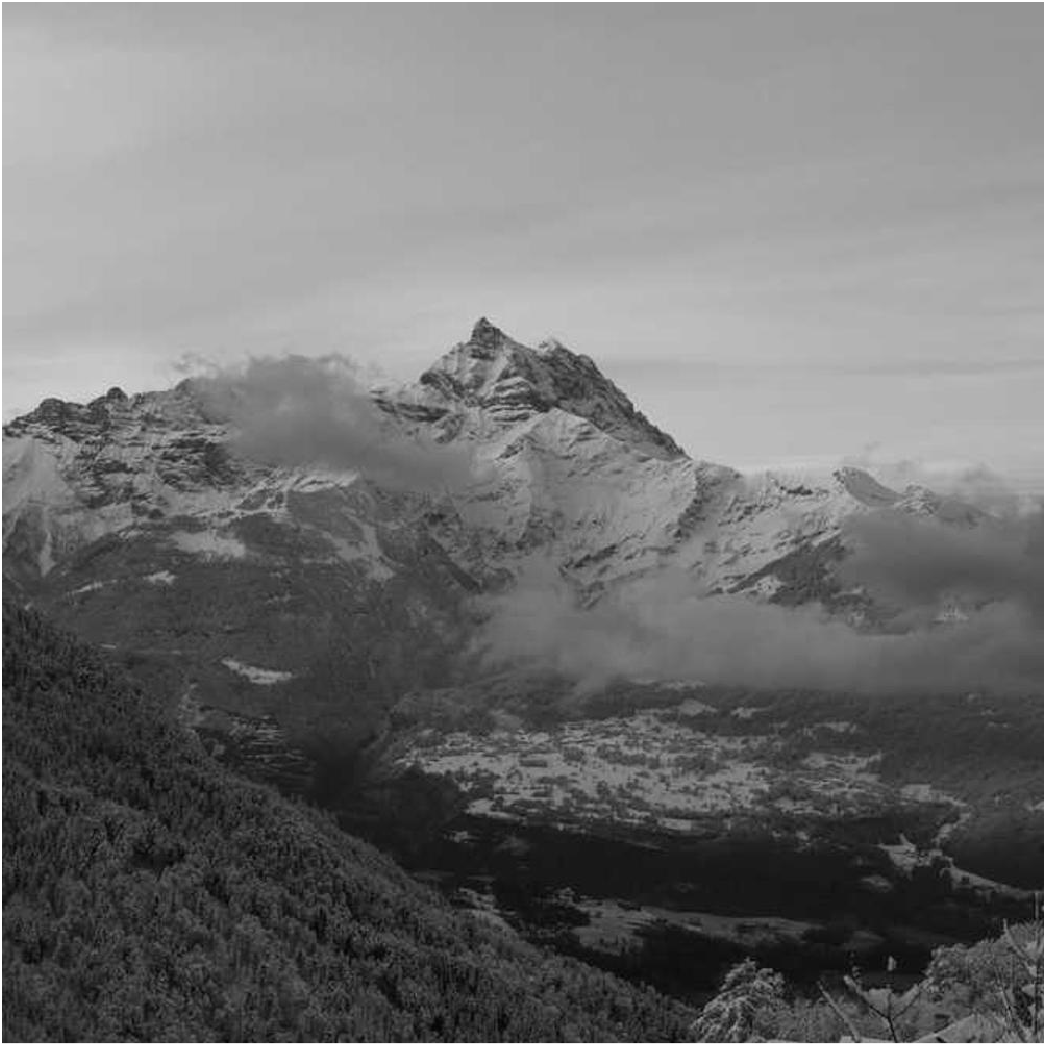
\includegraphics[width=\linewidth]{\mapa/slikaInput.png}
        \caption{Originalna slika.}
    \end{subfigure}
    \hfill
    \begin{subfigure}{0.49\linewidth}
        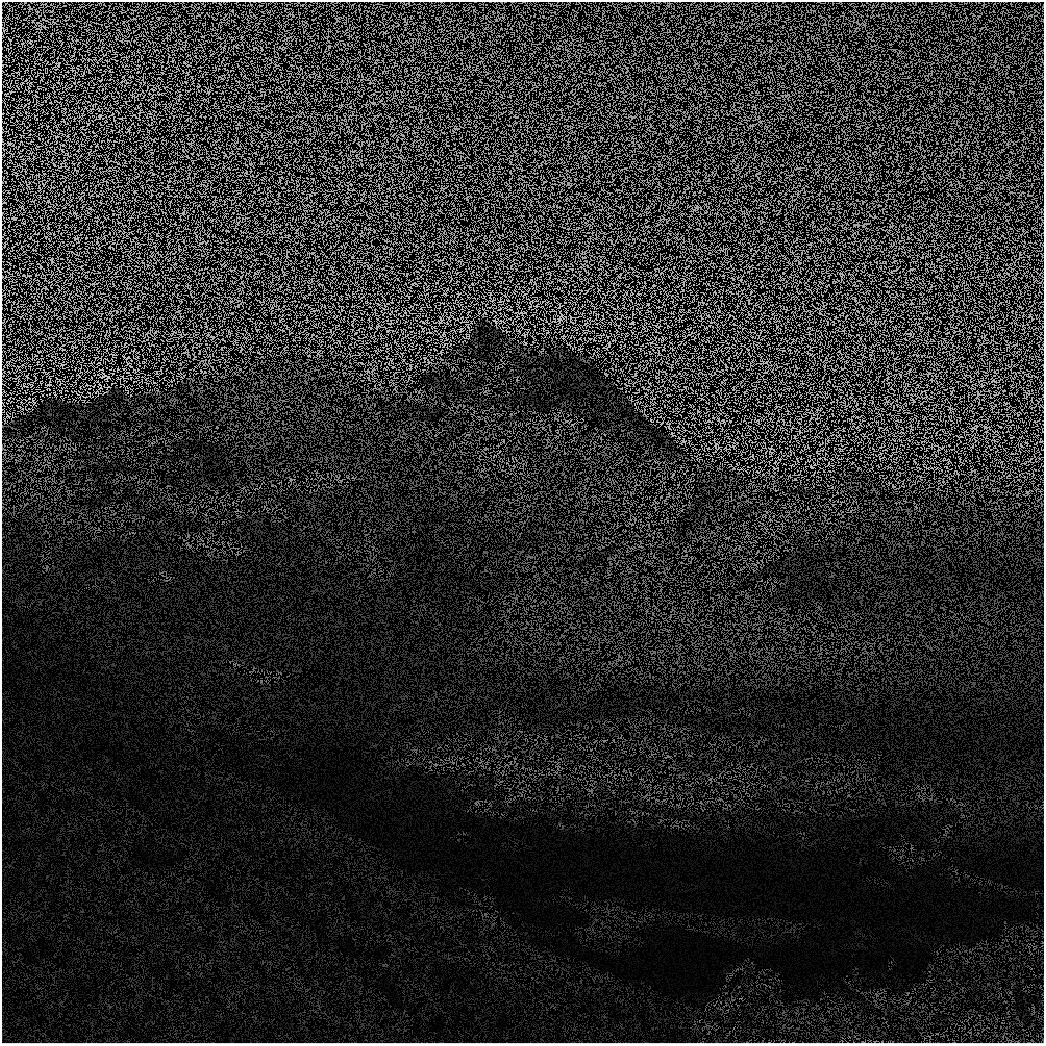
\includegraphics[width=\linewidth]{\mapa/slikaInput35.png}
        \caption{Slika z $35\%$ znanimi podatki.}
    \end{subfigure}
    \begin{subfigure}{0.49\linewidth}
        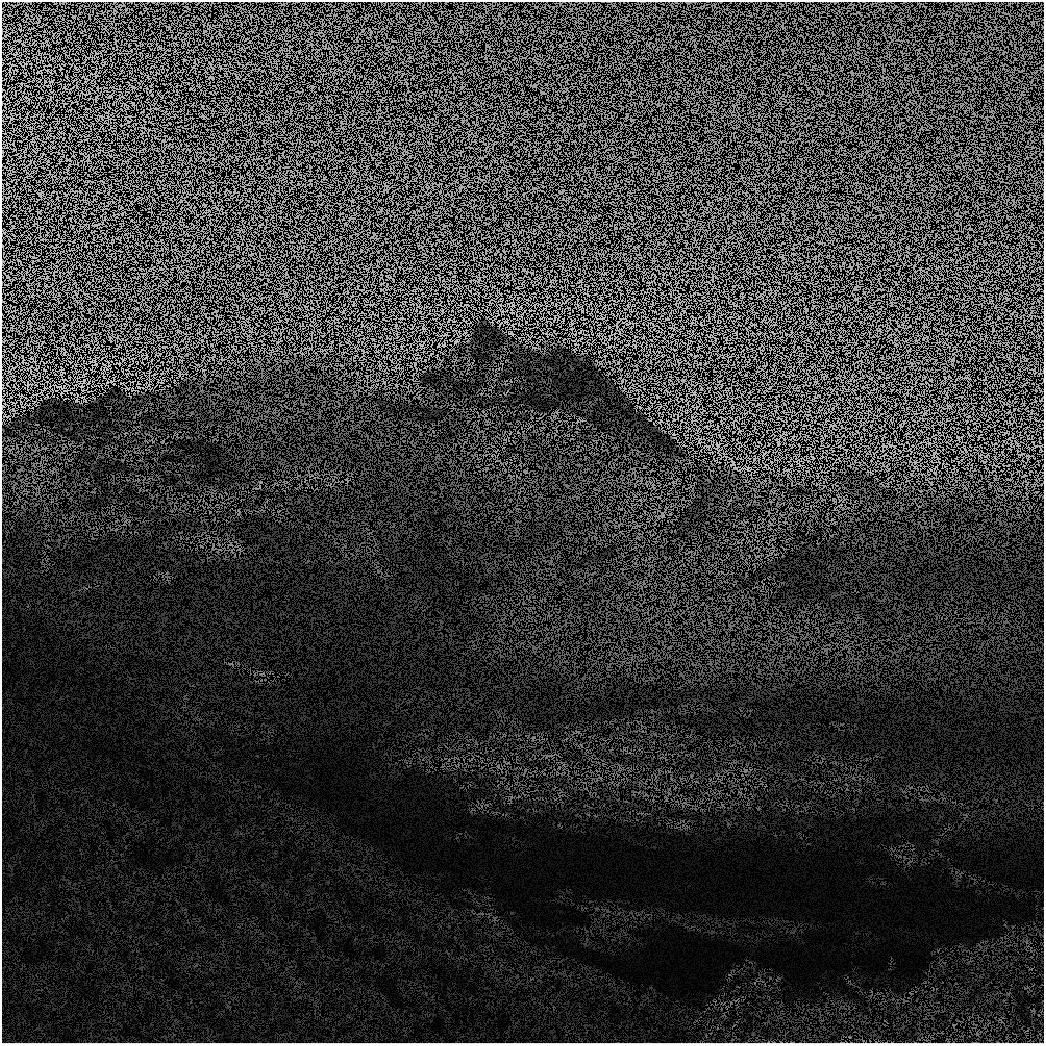
\includegraphics[width=\linewidth]{\mapa/slikaInput45.png}
        \caption{Slika z $45\%$ znanimi podatki.}
    \end{subfigure}
    \hfill
    \begin{subfigure}{0.49\linewidth}
        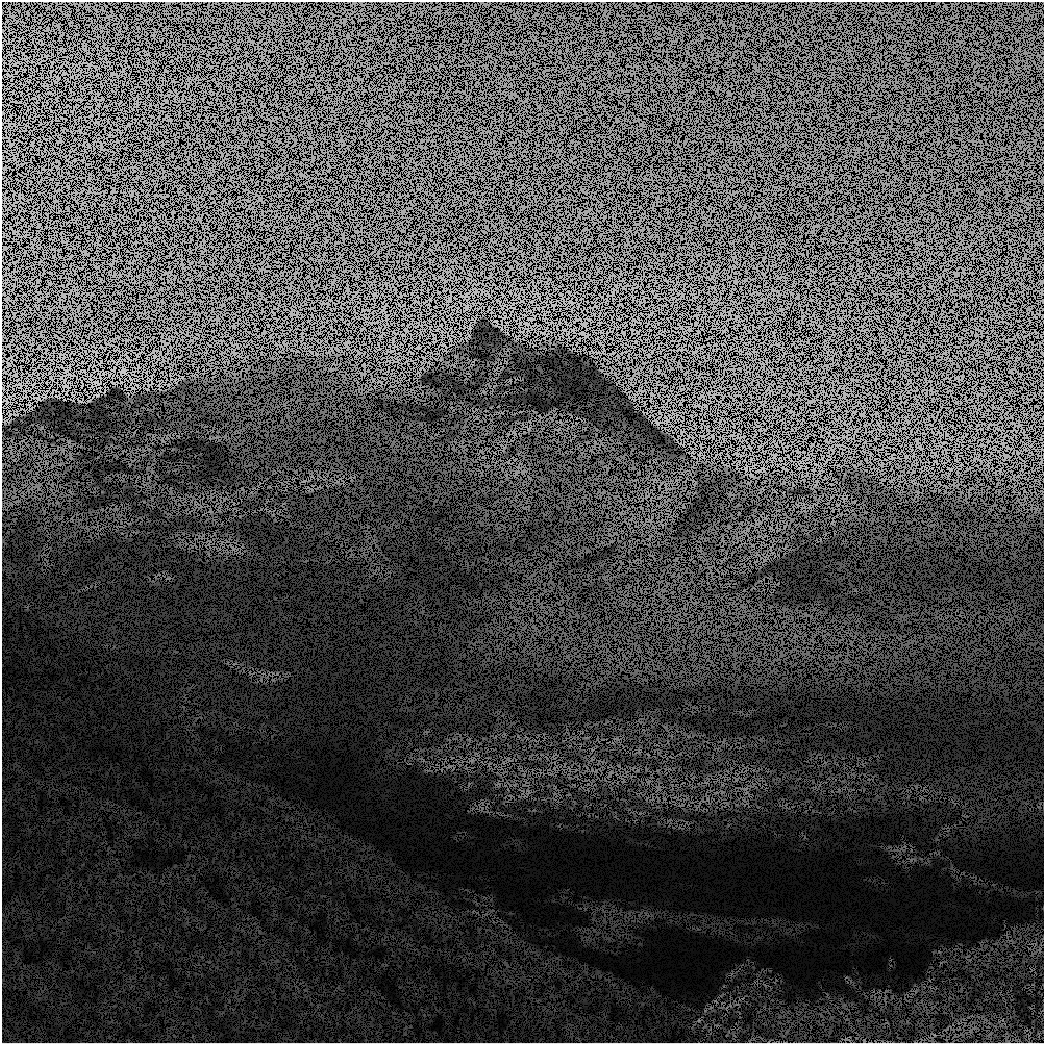
\includegraphics[width=\linewidth]{\mapa/slikaInput60.png}
        \caption{Slika z $60\%$ znanimi podatki.}
    \end{subfigure}
    \caption{Slika uporabljena za rekonstrukcijo. \cite{UnsplashGora}}
\end{figure}

\begin{figure}[!ht]
    \centering
    \begin{subfigure}{0.325\linewidth}
        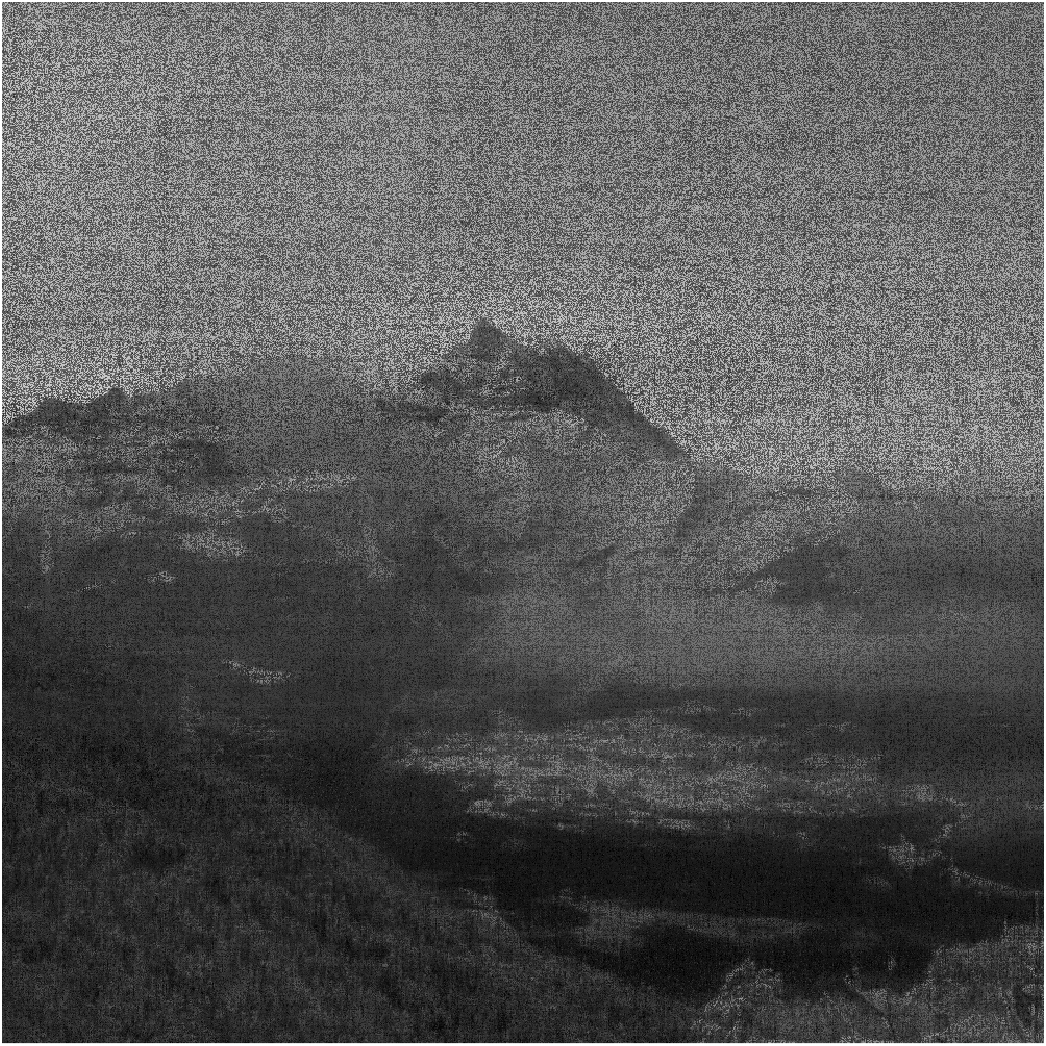
\includegraphics[width=\linewidth]{\mapa/slikaRez35SVT.png}
        \caption{SVT $35\%$}
    \end{subfigure}
    \hfill
    \begin{subfigure}{0.325\linewidth}
        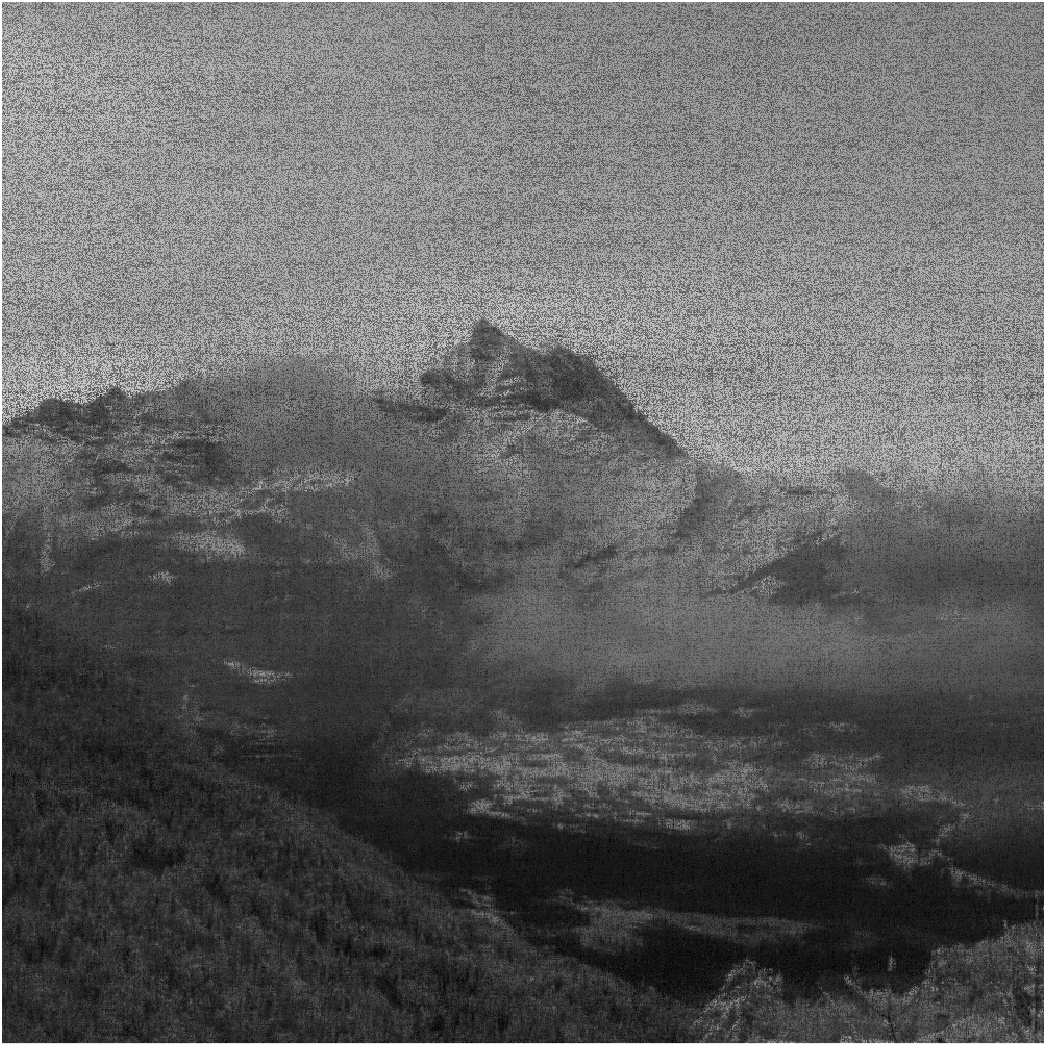
\includegraphics[width=\linewidth]{\mapa/slikaRez45SVT.png}
        \caption{SVT $45\%$}
    \end{subfigure}
    \hfill
    \begin{subfigure}{0.325\linewidth}
        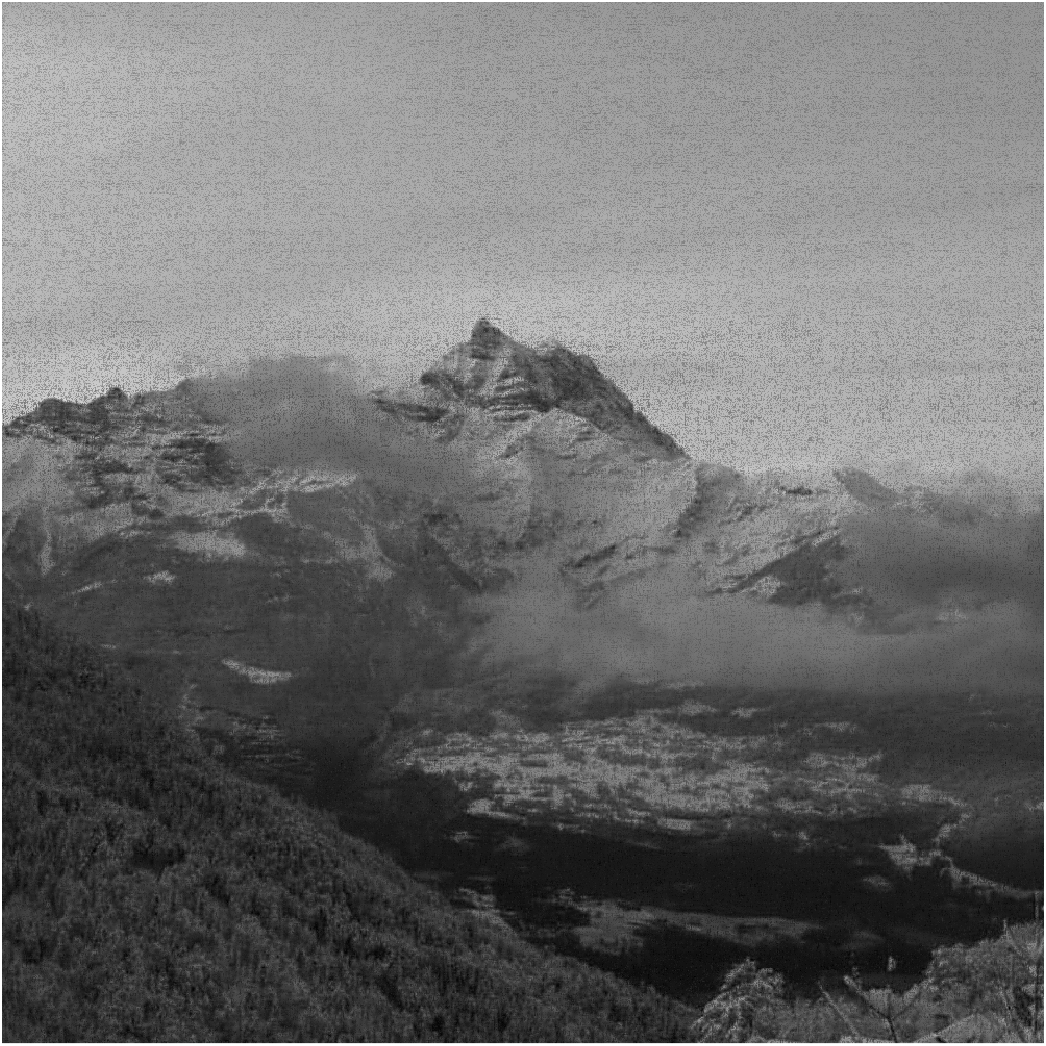
\includegraphics[width=\linewidth]{\mapa/slikaRez60SVT.png}
        \caption{SVT $60\%$}
    \end{subfigure}
    \begin{subfigure}{0.325\linewidth}
        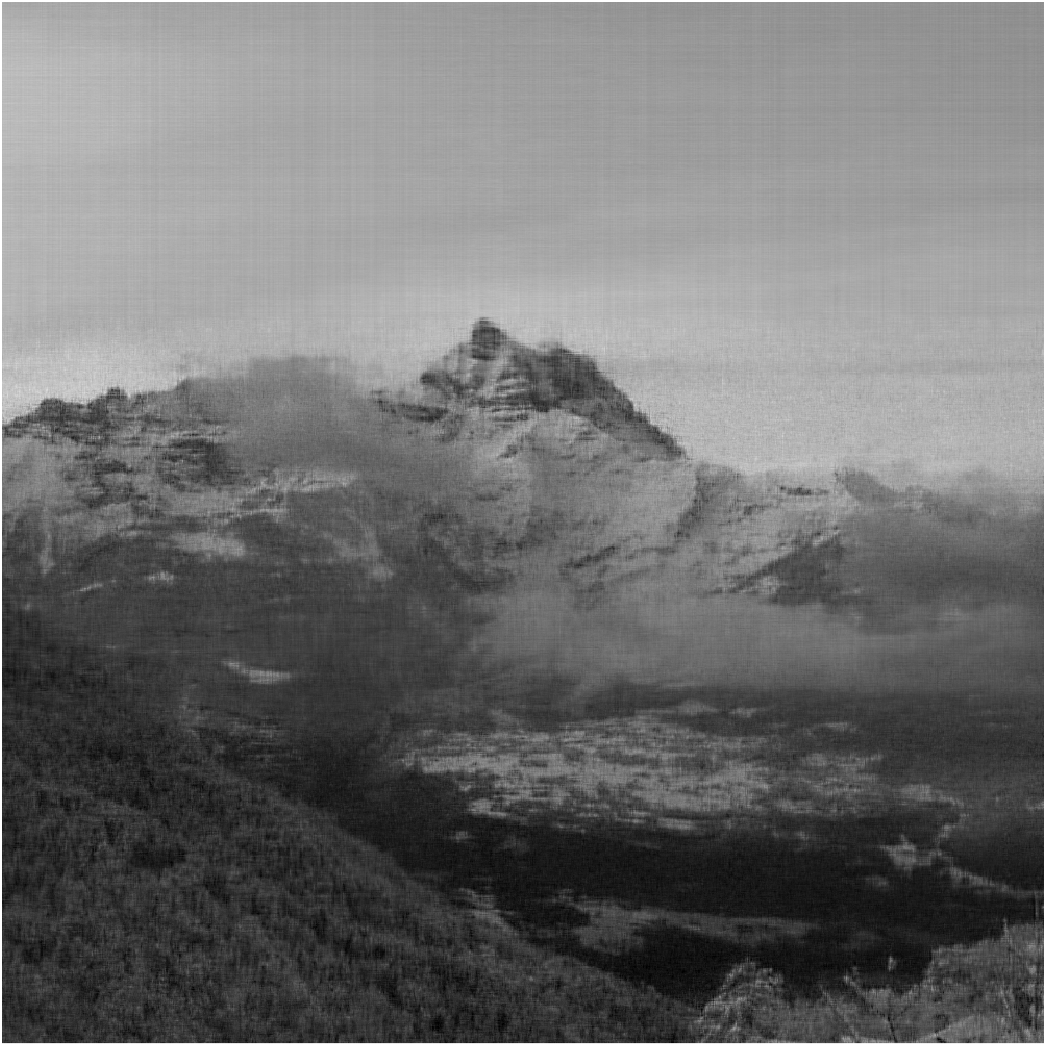
\includegraphics[width=\linewidth]{\mapa/slikaRez35TNNM.png}
        \caption{TNNM $35\%$}
    \end{subfigure}
    \hfill
    \begin{subfigure}{0.325\linewidth}
        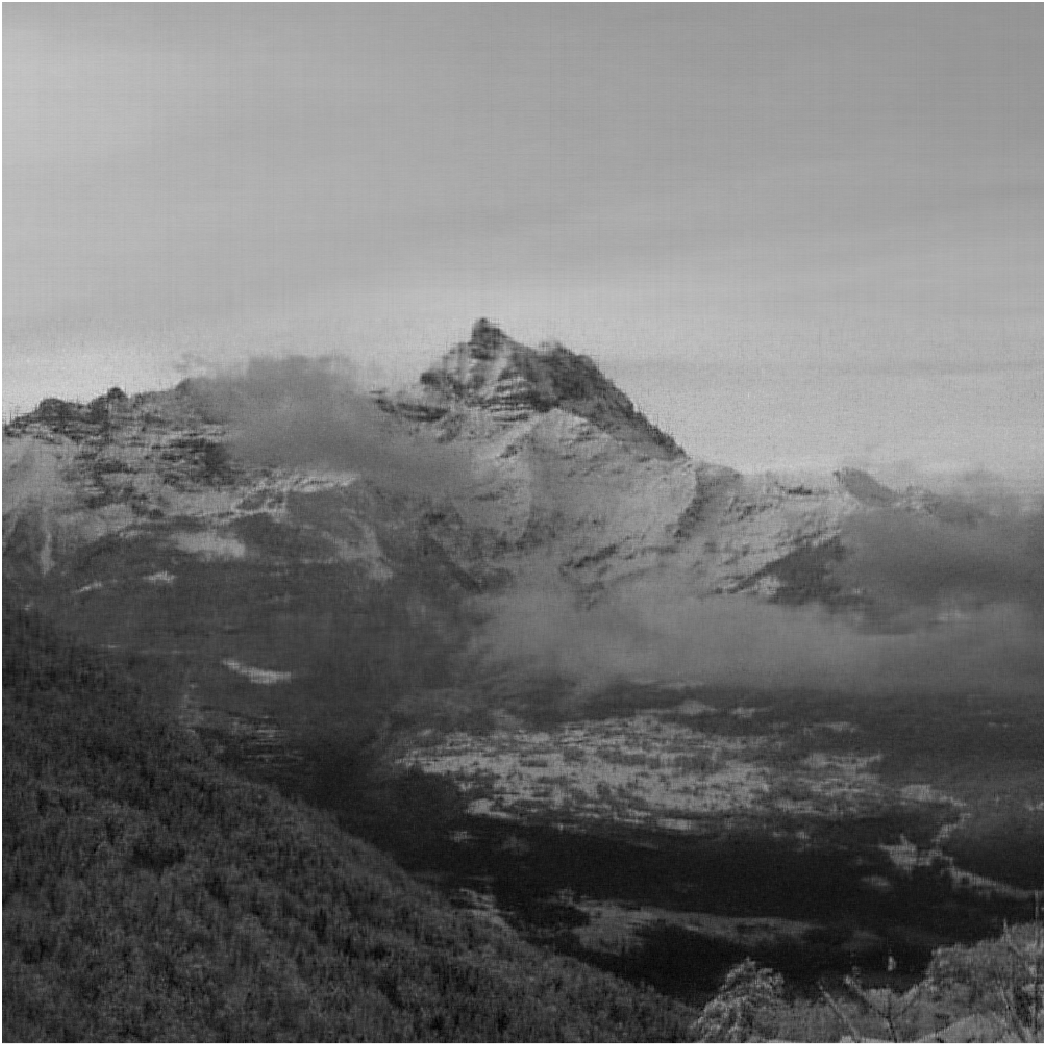
\includegraphics[width=\linewidth]{\mapa/slikaRez45TNNM.png}
        \caption{TNNM $45\%$}
    \end{subfigure}
    \hfill
    \begin{subfigure}{0.325\linewidth}
        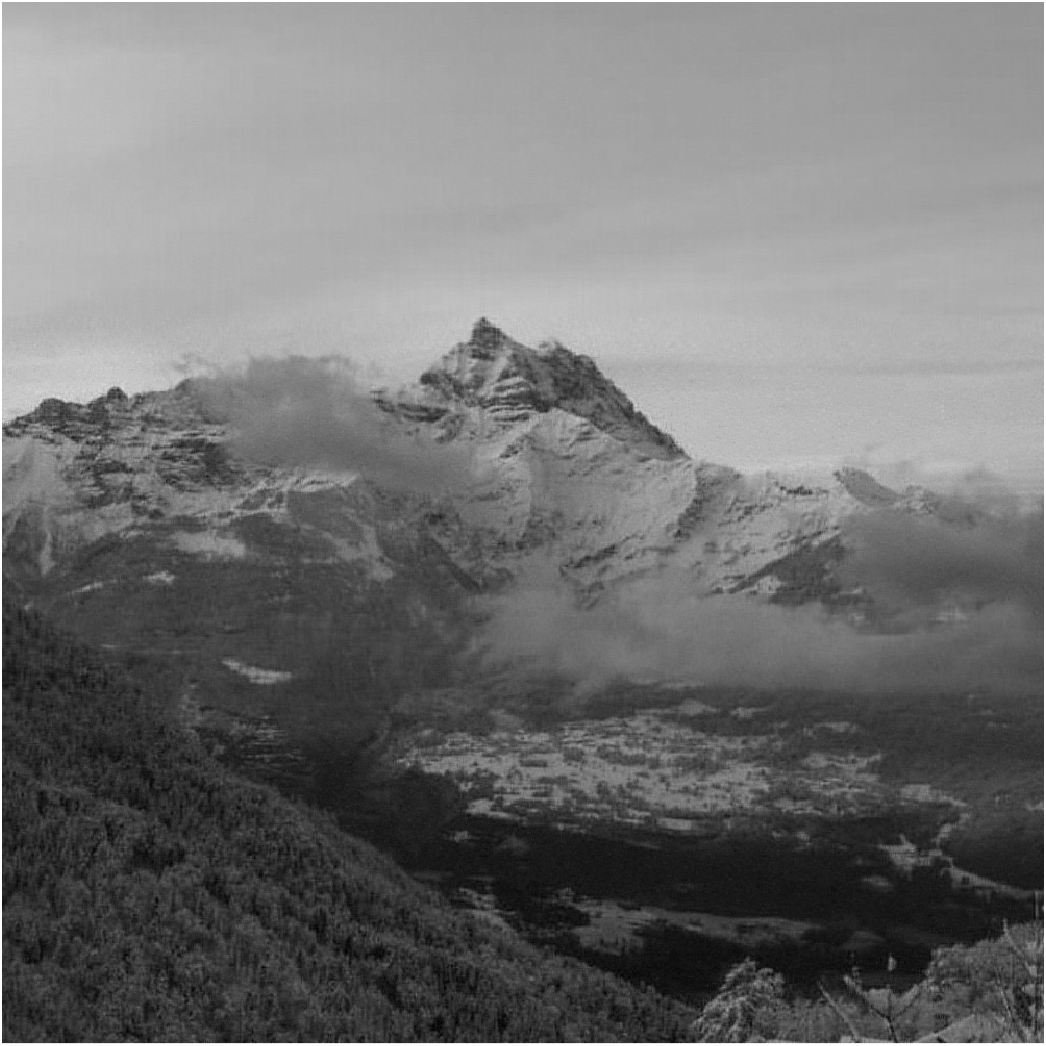
\includegraphics[width=\linewidth]{\mapa/slikaRez60TNNM.png}
        \caption{TNNM $60\%$}
    \end{subfigure}
    \begin{subfigure}{0.325\linewidth}
        
\includegraphics[width=\linewidth]{\mapa/slikaRez35ASD400.png}
        \caption{ASD $35\%$}
    \end{subfigure}
    \hfill
    \begin{subfigure}{0.325\linewidth}
        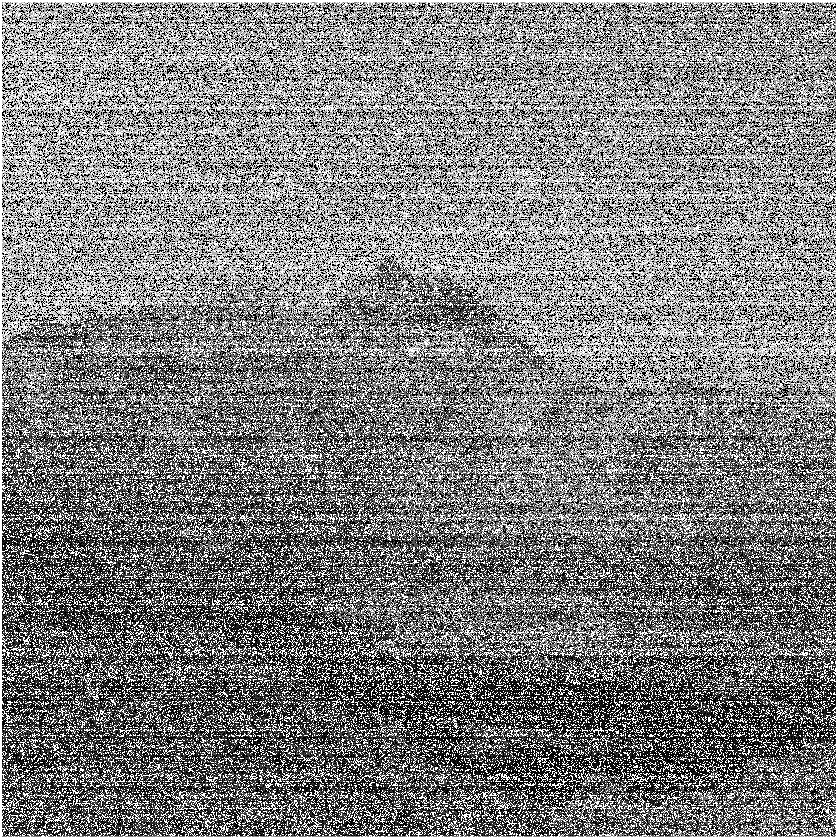
\includegraphics[width=\linewidth]{\mapa/slikaRez45ASD600.png}
        \caption{ASD $45\%$}
    \end{subfigure}
    \begin{subfigure}{0.325\linewidth}
        %ASD 60?%
        \hfill
    \end{subfigure}
    \begin{subfigure}{0.325\linewidth}
        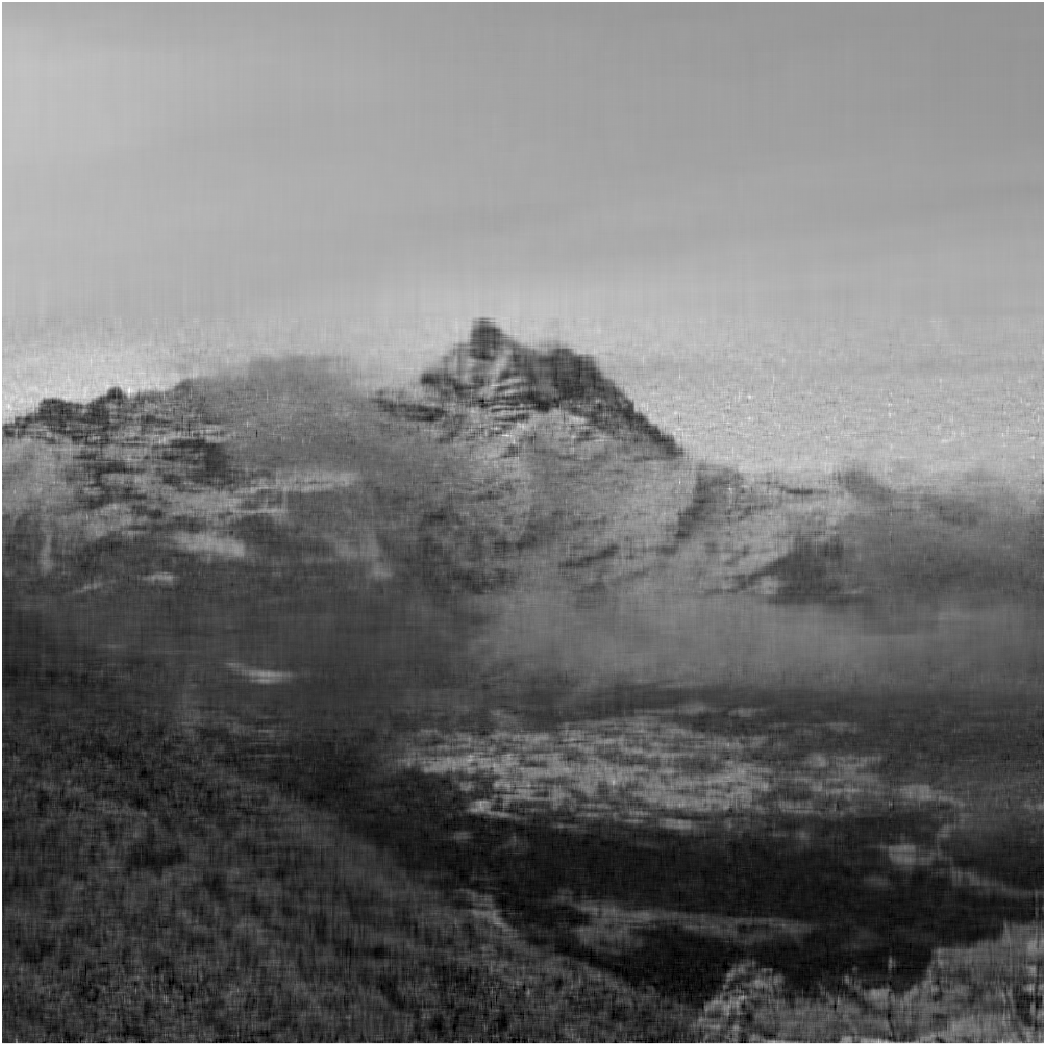
\includegraphics[width=\linewidth]{\mapa/slikaRez35LmaFIT50.png}
        \caption{LMaFit $35\%$}
    \end{subfigure}
    \hfill
    \begin{subfigure}{0.325\linewidth}
        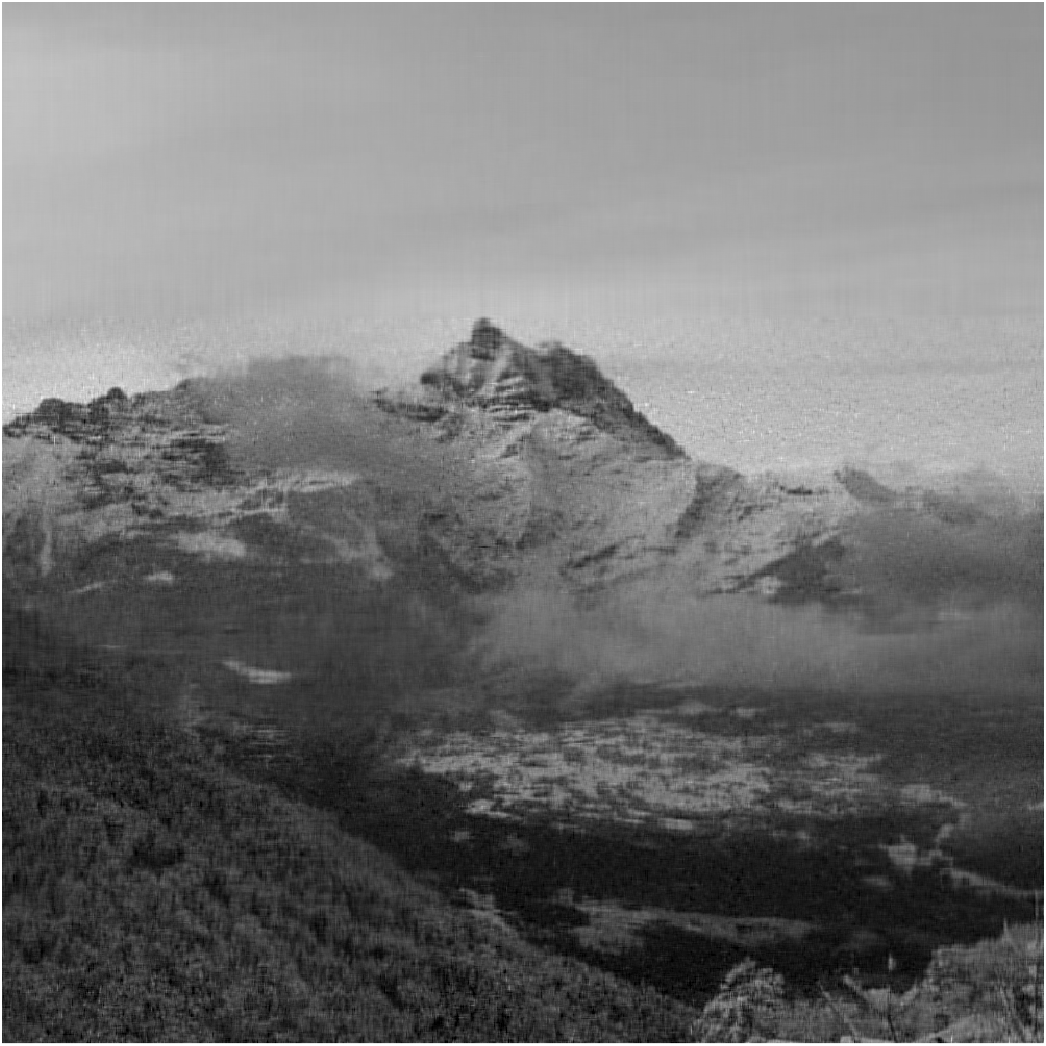
\includegraphics[width=\linewidth]{\mapa/slikaRez45LmaFIT73.png}
        \caption{LMaFit $45\%$}
    \end{subfigure}
    \begin{subfigure}{0.325\linewidth}
        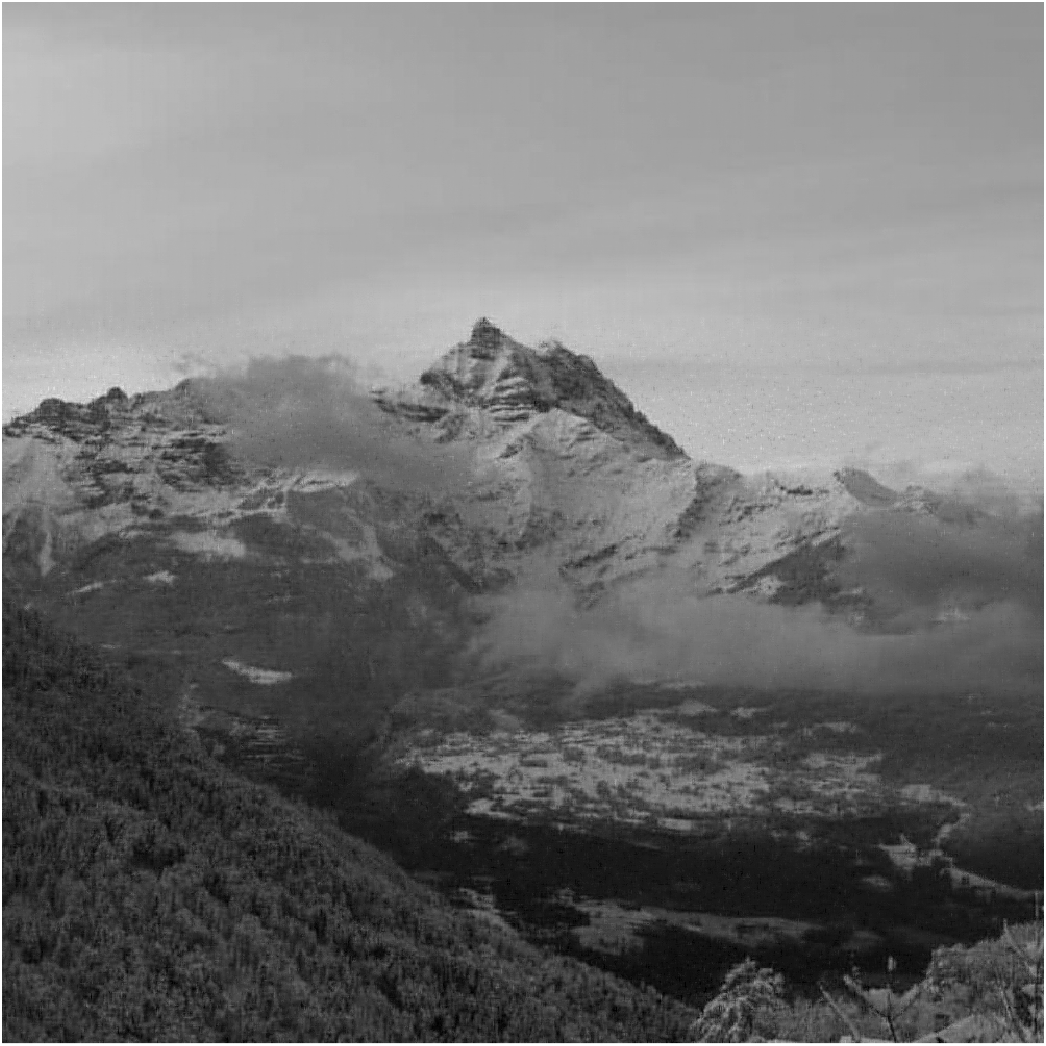
\includegraphics[width=\linewidth]{\mapa/slikaRez60LmaFIT77.png}
        \caption{LMaFit $60\%$}
    \end{subfigure}
\end{figure}
\FloatBarrier

Kot vidimo, je med rezultati velika razlika. Očitno je, da algoritmi TNNM, SVT in LMaFit delujejo najbolje, medtem ko ima algoritem ADDM vprašljive rezultate. Te si lahko interpretiramo kot posledico lastnosti, da lahko algoritem končata v lokalnem minimumu. Prav tako algoritem ADMM ni našel rešitve, ko je imel poznanih $0.60$ podatkov. Zato je ta algoritma smiselno uporabljati, kadar imamo dober začeten približek matrik $X$ in $Y$ ter manj poznanih vrednosti. Algoritem NNM smo med rezultati izpustili, saj je zaradi velikega števila matrik, potrebnih za definicijo omejitev, algoritem preveč prostorsko kompleksen. Ta algoritem bomo zato obravnavali posebej. Zaradi teh opazk se v naslednjih podpoglavjih v večini osredotočamo na algoritme SVT, TNNM in LMaFit.
\todo{je potrebno in graf in tabelo?}
\begin{table}[h]
    \centering
    \begin{tabular}{|c|c|c|c|c|}
    \hline
    & SVT & TNNM & LMAFIT & ASD \\ \hline
    0.35 & $4.69 \times 10^4$ & $7.70 \times 10^3$ & $8.03 \times 10^3$ & $3.9743 \times 10^7$ \\ \hline
    0.45 & $3.15 \times 10^4$ & $5.30 \times 10^3$ & $6.40 \times 10^3$ & $6.0910 \times 10^7$ \\ \hline
    0.6 & $1.25 \times 10^4$ & $3.58 \times 10^3$ & $5.35 \times 10^3$ & - \\ \hline
    \end{tabular}
\end{table}
\begin{figure}[!ht]
    \centering
    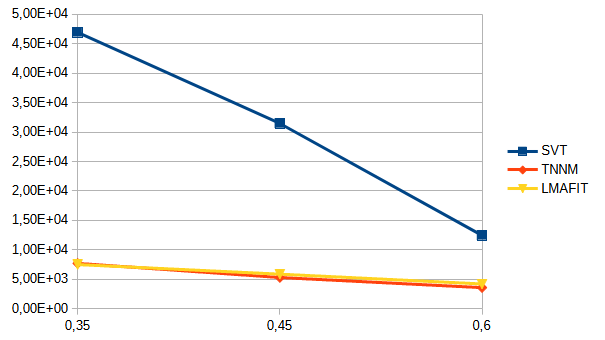
\includegraphics[width=\linewidth]{Poglavja/Slike/grayscale1000/grafNapake.png}
    \caption{Napake algoritmov glede na delež znanih vrednosti}
\end{figure}

\begin{table}[h]
    \centering
    \begin{tabular}{|c|c|c|c|c|}
    \hline
    & SVT & TNNM & LMAFIT & ASD \\ \hline
    0.35 & 338s & 824s & 235s & 1012s \\ \hline
    0.45 & 510s & 498s & 342s & 328s\\ \hline
    0.6 & 1674s & 350s & 48s & - \\ \hline
    \end{tabular}
\end{table}
\begin{figure}[!ht]
    \centering
    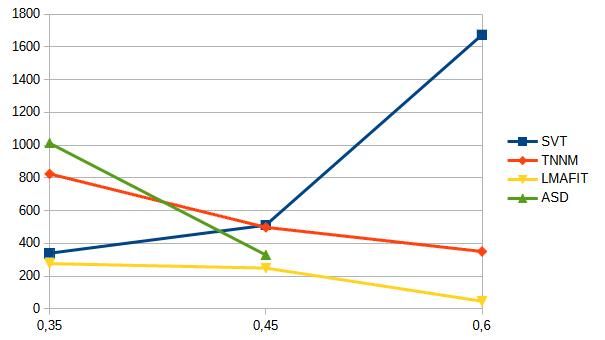
\includegraphics[width=\linewidth]{Poglavja/Slike/grayscale1000/grafCas.png}
    \caption{Časi izvajanja algoritmov glede na delež znanih vrednosti}
\end{figure}

\section{Vpliv kompleksnosti slik na napolnjevanje}
Eno izmed glavnih vprašanj, ki se nam lahko porodi pri implementaciji algoritmov za napolnitev matrik je, kako sama kompleksnost slik vpliva na točnost rezultatov. Ker slike naključnih vrednosti ni mogoče rekonstruirati, lahko sklepamo, da bodo slike s preprostimi motivi napolnjene bolje. Za namene testiranja je torej smiselno izbrati tako preprosto kot tudi vizualno nasičeno sliko. V naših testiranjih uporabljamo sliki knjige in mesta. Sliki sta velikosti $300 \times 300$ pikslov
\renewcommand{\mapa}{Poglavja/Slike/kompleksnost}

\begin{figure}[!ht]
    \begin{subfigure}{0.5\linewidth}
        
\includegraphics[width=\linewidth]{\mapa/preprosta grayscale 300/knjiga.png}
        \caption{Slika s preprostim motivom.}
    \end{subfigure}
    \hfill
    \begin{subfigure}{0.5\linewidth}
        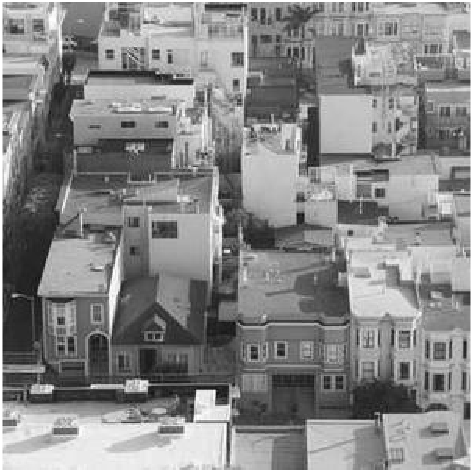
\includegraphics[width=\linewidth]{\mapa/kompleksna grayscale 300/mesto.png}
        \caption{Slika s kompleksnim motivom.}
    \end{subfigure}
    \caption{Vira slik: \cite{UnsplashKnjiga,UnsplashMesto}.}
\end{figure}

\begin{figure}[!ht]
    \begin{subfigure}{0.325\linewidth}
        \includegraphics[width=\linewidth]{\mapa/preprosta grayscale 300/rez35SVT.png}
    \end{subfigure}
    \hfill
    \begin{subfigure}{0.325\linewidth}
        
\includegraphics[width=\linewidth]{\mapa/preprosta grayscale 300/rez45SVT.png}
    \end{subfigure}
    \hfill
    \begin{subfigure}{0.325\linewidth}
        \includegraphics[width=\linewidth]{\mapa/preprosta grayscale 300/rez60SVT.png}
    \end{subfigure}
    \caption{Rekonstrukcija preprostega motiva z algoritmom SVT. Odstotki znanih vrednosti slik so bili 35\% (leva), 45\% (sredinska) in 60\% (desna).
    }
\end{figure}
    
\begin{figure}[!ht]
    \begin{subfigure}{0.325\linewidth}
        \includegraphics[width=\linewidth]{\mapa/kompleksna grayscale 300/rez35SVT.png}
    \end{subfigure}
    \hfill
    \begin{subfigure}{0.325\linewidth}
        
\includegraphics[width=\linewidth]{\mapa/kompleksna grayscale 300/rez45SVT.png}
    \end{subfigure}
    \hfill
    \begin{subfigure}{0.325\linewidth}
        \includegraphics[width=\linewidth]{\mapa/kompleksna grayscale 300/rez60SVT.png}
    \end{subfigure}
    \caption{Rekonstrukcija kompleksnega motiva z algoritmom SVT. Odstotki znanih vrednosti slik so bili 35\% (leva), 45\% (sredinska) in 60\% (desna).}
\end{figure}

\begin{figure}[!ht]
    \begin{subfigure}{0.325\linewidth}
        \includegraphics[width=\linewidth]{\mapa/preprosta grayscale 300/rez35TNNM.png}
    \end{subfigure}
    \hfill
    \begin{subfigure}{0.325\linewidth}
        
\includegraphics[width=\linewidth]{\mapa/preprosta grayscale 300/rez45TNNM.png}
    \end{subfigure}
    \hfill
    \begin{subfigure}{0.325\linewidth}
        \includegraphics[width=\linewidth]{\mapa/preprosta grayscale 300/rez60TNNM.png}
    \end{subfigure}
    \caption{Rekonstrukcija preprostega motiva z algoritmom TNNM. Odstotki znanih vrednosti slik so bili 35\% (leva), 45\% (sredinska) in 60\% (desna).}
\end{figure}

\begin{figure}[!ht]
    \begin{subfigure}{0.325\linewidth}
        \includegraphics[width=\linewidth]{\mapa/kompleksna grayscale 300/rez35TNNM.png}
    \end{subfigure}
    \hfill
    \begin{subfigure}{0.325\linewidth}
        
\includegraphics[width=\linewidth]{\mapa/kompleksna grayscale 300/rez45TNNM.png}
    \end{subfigure}
    \hfill
    \begin{subfigure}{0.325\linewidth}
        \includegraphics[width=\linewidth]{\mapa/kompleksna grayscale 300/rez60TNNM.png}
    \end{subfigure}
    \caption{Rekonstrukcija kompleksnega motiva z algoritmom TNNM. Odstotki znanih vrednosti slik so bili 35\% (leva), 45\% (sredinska) in 60\% (desna).}
\end{figure}

\begin{figure}[!ht]
    \begin{subfigure}{0.325\linewidth}
        \includegraphics[width=\linewidth]{\mapa/preprosta grayscale 300/rez35LMaFit.png}
    \end{subfigure}
    \hfill
    \begin{subfigure}{0.325\linewidth}
        \includegraphics[width=\linewidth]{\mapa/preprosta grayscale 300/rez45LMaFit.png}
    \end{subfigure}
    \hfill
    \begin{subfigure}{0.325\linewidth}
        \includegraphics[width=\linewidth]{\mapa/preprosta grayscale 300/rez60LMaFit.png}
    \end{subfigure}
    \caption{Rekonstrukcija preprostega motiva z algoritmom LMaFit. Odstotki znanih vrednosti slik so bili 35\% (leva), 45\% (sredinska) in 60\% (desna).}
\end{figure}

\begin{figure}[!ht]
    \begin{subfigure}{0.325\linewidth}
        \includegraphics[width=\linewidth]{\mapa/kompleksna grayscale 300/rez35LMaFit.png}
    \end{subfigure}
    \hfill
    \begin{subfigure}{0.325\linewidth}
        \includegraphics[width=\linewidth]{\mapa/kompleksna grayscale 300/rez45LMaFit.png}
    \end{subfigure}
    \hfill
    \begin{subfigure}{0.325\linewidth}
        \includegraphics[width=\linewidth]{\mapa/kompleksna grayscale 300/rez60LMaFit.png}
    \end{subfigure}
    \caption{Rekonstrukcija preprostega motiva z algoritmom LMaFit. Odstotki znanih vrednosti slik so bili 35\% (leva), 45\% (sredinska) in 60\% (desna).}
\end{figure}
\todo{Lmafit vcasih potrebno zagnati veckat}
\begin{figure}[!ht]
    \centering
    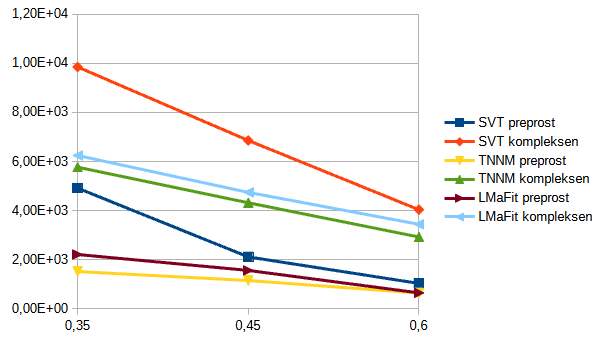
\includegraphics[width=\linewidth]{Poglavja/Slike/kompleksnost/kompleksna grayscale 300/kompleksnost.png}
    \caption{Graf napak algoritmov}
\end{figure}

Kot smo pričakovali, so rezultati rekonstrukcije slike s preprostim motivom boljše. Prav tako lahko opazimo, da ima delež znanih vrednosti močnejši vpliv pri sliki s kompleksnim motivom. Napake z dodajanjem informacij torej hitreje padajo pri matrikah večjega ranga. Spomnimo se, da algoritma LMaFit in TNNM za svoje delovanje potrebujeta informacijo o rangu. Pri testiranju je bilo zato potrebno kompleksni sliki podati večjo vrednost ranga, da sta lahko algoritma prišla do dobrih rezultatov.

Sama točnost algoritmov pa ostaja zelo podobna rekonstrukciji velike slike, torej z najboljšimi rezultati pridobljenimi z algoritmom TNNM, nato LMaFit in z najslabšimi rezultati algoritem SVT.

\begin{figure}[!ht]
    \centering
    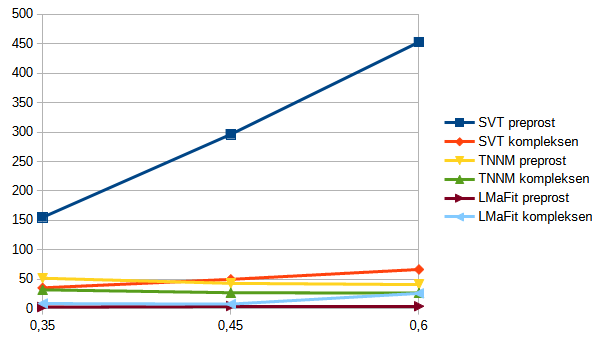
\includegraphics[width=\linewidth]{Poglavja/Slike/kompleksnost/kompleksna grayscale 300/cas.png}
    \caption{Graf časov izvajanja algoritmov}
\end{figure}
Sami časi izvajanja pa tu niso tako intuitivni. Prva glavna opazka je, da algoritem SVT potrebuje veliko več časa pri preprostem motivu kot pri kompleksem. \todo{razmisli to interpretacijo} To si lahko razlagamo kot posledico praga. Za dobre rezultate smo pri tako majhni matriki prag nastavili visoko. V našem primeru je imel ta vrednost $3600$. V primeru preprostega motiva, lahko pričakujemo, da bomo imeli malo zelo velikih singularnih vrednosti. Zaradi tega se algoritem težko premika in išče rešitev. Iz tega sledi opazka, da je algoritem SVT bolj smiselno uporabljati za kompleksne motive.

Naslednja pomembna opazka pa je, da delež znanih vrednosti različno vpliva na sam čas izvajanja. Tudi ta faktor je torej lahko pomemben pri izbiri algoritma za reševanje problema. Algoritem SVT potrebuje za rekonstrukcijo več časa, kadar ima poznanih več vrednosti, medtem ko se algoritmu TNNM z deležem znanih vrednosti čas izvajanja manjša. Algoritmu LMaFit težko določimo pravilo, saj najpočasnejše izvede rekonstrukcijo pri $0.45$ znanih podatkov. Iz tega sklepamo, da je pri nekem deležu med $0.35$ in $0.6$ rekonstrukcija najpočasnejša. Tu pa je vredno tudi omeniti, da zaradi naključnega generiranja začetne matrike algoritem lahko različno dolgo rekonstruira isti primer. \todo{Preveri znova} Ker pa smo teste pognali večkrat ter v povprečju vedno najdlje čakali pri vrednosti $0.45$ lahko sklepamo, da je v takih primerih rekonstrukcija res bolj zahtevna.

\section{Rekonstrukcija barvnih slik}
Naslednje vprašanje, ki se nam lahko porodi pri testiranju algoritmov je, kako vplivajo barvne slike na samo rekonstrukcijo. Barvne slike so podatkovno podane kot kombinacija barvnih kanalov rdeče, zelene in modre barve. Glavno vprašanje, na katerega bomo poskušali odgovoriti v tem poglavju je, ali je bolje napolnjevati vsak barvni kanal posebej, ali sliko kot celotno. V prvem primeru torej algoritem zaženemo trikrat, medtem ko v drugem sestavimo veliko matriko sestavljeno kot 
\[
    A = \begin{bmatrix}
        R\\G\\B
    \end{bmatrix} 
\] 
kjer $R$ predstavlja matriko z vrednostmi rdečega kanala, G vrednosti zelenega kanala ter B vrednosti modrega kanala.
Vsi testi v tej fazi so bili izvedeni na podatkih, kjer imamo poznanih $0.35$ informacij.
\todo{kako omeniti da je frobenius}
\begin{table}[h]
    \centering
    \begin{tabular}{|c|c|c|c|}
    \hline
    & SVT & TNNM & LMAFIT \\
    \hline
    Enojna rekonstrukcija & $1,50 \times 10^4$ & $9,60\times 10^3$ & $1,15\times 10^4$ \\
    Trojna rekonstrukcija & $1,66\times 10^4$ & $9,79\times 10^3$ & $1,14\times 10^4$ \\
    \hline
    \end{tabular}
\end{table}

\begin{table}[h]
    \centering
    \begin{tabular}{|c|c|c|c|}
    \hline
    & SVT & TNNM & LMAFIT \\
    \hline
    Enojna rekonstrukcija & 352s & 124s & 66s \\
    Trojna rekonstrukcija & 112s & 100s & 42s \\
    \hline
    \end{tabular}
\end{table}
Lahko je videti, da medtem ko obe metodi vrnete približno enako dobre rezultate, je rekonstrukcija pri vseh algoritmih hitrejša, če ločene barvne kanale rekonstruiramo posebej. Iz tu je lahko videti, da je smiselno med sabo neodvisne podatke ločiti, ter jih reševati samostojno. Rezultat je smiselen, saj nam iskanje podobnosti med nepodobnimi podatki poveča količino dela. 

\section{Vpliv podatka o rangu na rezultate}
Kot smo omenili že nekajkrat, algoritma TNNM in LMaFit za svoje izvajanje potrebujeta informacijo o rangu (v nadaljevanju parameter). V tem podpoglavju bomo poskušali odgovoriti na vprašanje, kako pri obeh algoritmih ta informacija vpliva na same rezultate in izvajanje. Za namene testiranja smo algoritem na isti sliki pognali večkrat, ter postopoma večali rang. Ponovno smo teste izvajali na sliki mesta, z znanim deležem podatkov nastavljenim na $0,35$.

\subsection{LMaFit}
V tej fazi smo algoritem testirali štirikrat, z rangom rezultata določenega na
$1, 5, 10, 22, 25$ in $60$. Vrednost $22$ je bila izbrana, ker je ob večkratnem zagonu programa na različnih parametrih, ta dala najboljši rezultat. Posledično sta bili vrednosti $25$ in $60$ izbrani z namenom opazovanja, kakšne rezultate pridobimo s precenitvijo ranga rekonstruirane matrike. 
\renewcommand{\mapa}{Poglavja/Slike/informacija ranga}

\begin{figure}[!ht]
    \begin{subfigure}{0.325\linewidth}
        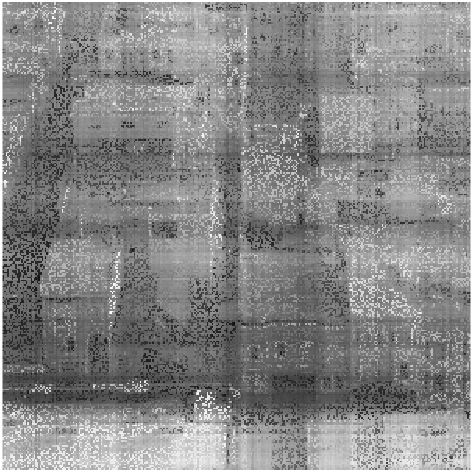
\includegraphics[width=\linewidth]{\mapa/rezLMaFit1.png}
        \caption{Rekonstrukcija s parametrom 1.}
    \end{subfigure}
    \hfill
    \begin{subfigure}{0.325\linewidth}
        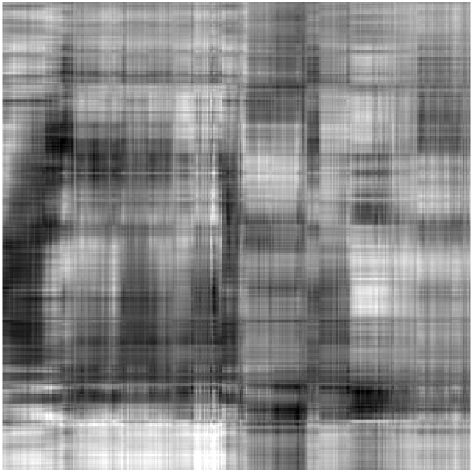
\includegraphics[width=\linewidth]{\mapa/rezLMaFit5.png}
        \caption{Rekonstrukcija s parametrom 5.}
    \end{subfigure}
    \hfill
    \begin{subfigure}{0.325\linewidth}
        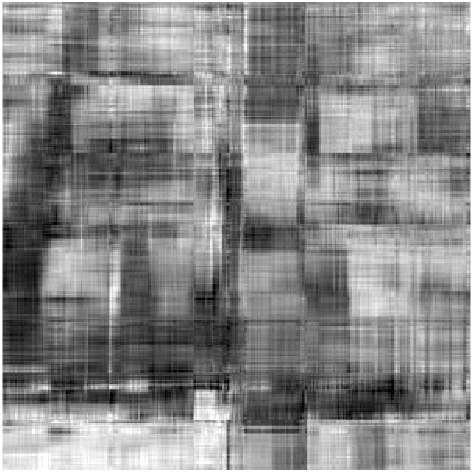
\includegraphics[width=\linewidth]{\mapa/rezLMaFit10.png}
        \caption{Rekonstrukcija s parametrom 10.}
    \end{subfigure}

    \begin{subfigure}{0.325\linewidth}
        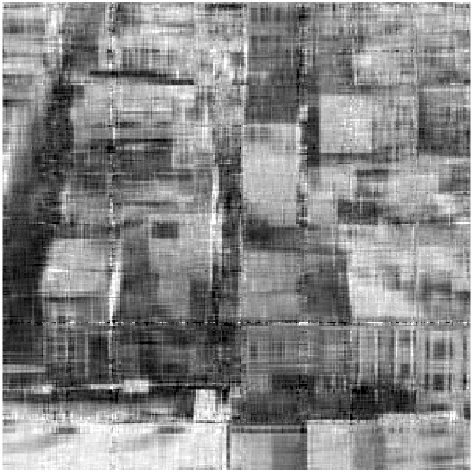
\includegraphics[width=\linewidth]{\mapa/rezLMaFit22.png}
        \caption{Rekonstrukcija s parametrom 22.}
    \end{subfigure}
    \hfill
    \begin{subfigure}{0.325\linewidth}
        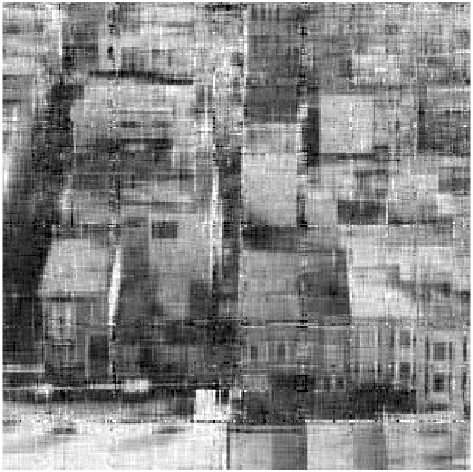
\includegraphics[width=\linewidth]{\mapa/rezLMaFit25.png}
        \caption{Rekonstrukcija s parametrom 25.}
    \end{subfigure}
    \hfill
    \begin{subfigure}{0.325\linewidth}
        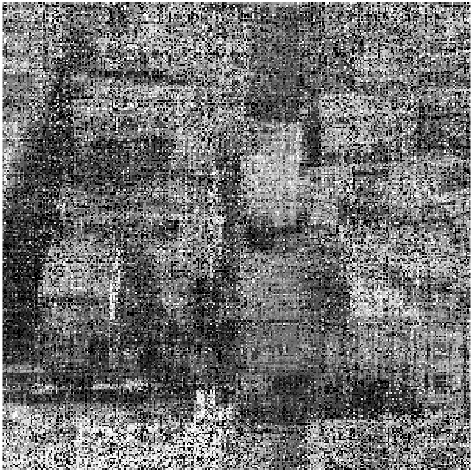
\includegraphics[width=\linewidth]{\mapa/rezLMaFit60.png}
        \caption{Rekonstrukcija s parametrom 60.}
    \end{subfigure}
\end{figure}

\begin{table}[h]
    \centering
    \begin{tabular}{|c|c|c|}
        \hline
        Parameter & Napaka (v $\fnorm{\cdot}$)& Čas izvajanja \\
        \hline
        1         & $1.11 \times 10^4$ & 0.04s        \\
        5         & $8.05 \times 10^3$ & 0.41s         \\
        10        & $6.61 \times 10^3$ & 0.42s        \\
        22        & $6.25 \times 10^3$ & 8.78s       \\
        25        & $6.57 \times 10^3$ & 41.26s        \\
        60        & $2.40 \times 10^4$ & 325.31s        \\
        \hline
    \end{tabular}
    \caption{Rezultati rekonstrukcije algoritma LMaFit za različne parametre.}
\end{table}


Opazimo lahko izboljševanje podrobnosti slike, vse do parametra $22$. Vidimo pa lahko tudi, da pride pri prevelikem parametru do preobrata. Rezultati se ponovno slabšajo, algoritem pa postane počasnejši. Iz tega lahko razberemo, da je pravilna izbira parametra ključna. Vredno je omeniti, da za vrednosti parametra na nekem intervalu algoritem ne konvergira. V primeru zgornje slike in parametra $30$, algoritem LMaFit ni našel rešitve. 

\subsection{TNNM}
Zaradi večje časovne zahtevnosti, algoritem TNNM testiramo zgolj trikrat, na deležih informacij $1, 5$ in $12$. Za večje parametre je algoritem konvergiral zelo počasi, zaradi česar se testiranjem teh izognemo. Tukaj se je pomembno spomniti, da parameter pri algoritmu TNNM ne določa samega ranga rezultata, vendar je zgolj povezan z njim pri reševanju, saj uporablja matriki $A_l$ in $B_l$. Zaradi tega je težje določiti pravilo, kateri parameter je najboljši.
\renewcommand{\mapa}{Poglavja/Slike/informacija ranga}
\begin{figure}[!ht]
    \begin{subfigure}{0.325\linewidth}
        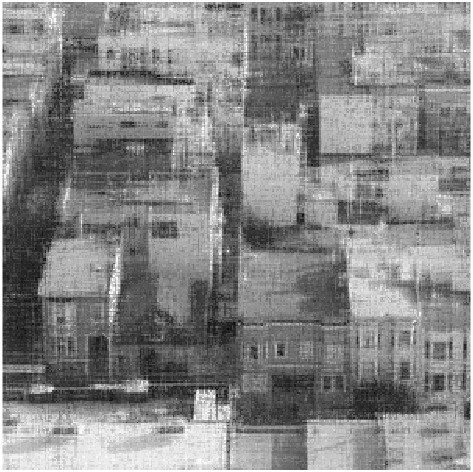
\includegraphics[width=\linewidth]{\mapa/rezTNNM1.png}
        \caption{Rekonstrukcija s parametrom 1.}
    \end{subfigure}
    \hfill
    \begin{subfigure}{0.325\linewidth}
        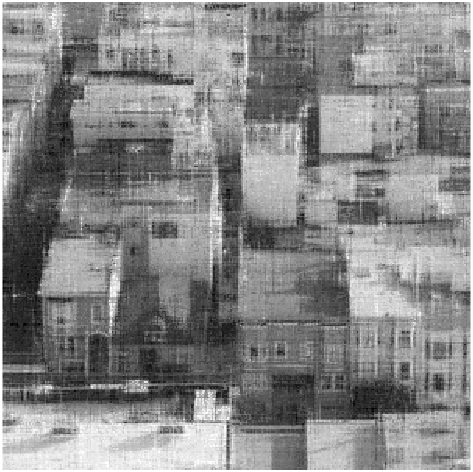
\includegraphics[width=\linewidth]{\mapa/rezTNNM5.png}
        \caption{Rekonstrukcija s parametrom 5.}
    \end{subfigure}
    \hfill
    \begin{subfigure}{0.325\linewidth}
        \includegraphics[width=\linewidth]{\mapa/rezTNNM12.png}
        \caption{Rekonstrukcija s parametrom 12.}
    \end{subfigure}
\end{figure}

\begin{figure}[h]
    \centering
    \begin{tabular}{|c|c|c|}
        \hline
        Parameter & Napaka (v $\fnorm{\cdot}$) & Čas izvajanja \\
        \hline
        1 & $5.70 \times 10^{3}$ & 35.9s \\
        5 & $5.46 \times 10^{3}$ & 481s \\
        12 & $5.27 \times 10^{3}$ & 930s \\
        \hline
    \end{tabular}
    \caption{Rezultati rekonstrukcije algoritma TNNM za različne parametre.}
\end{figure}


Sami rezultati med seboj delujejo podobni. Izračun napak nam pokaže, da medtem ko se napaka zmanjšuje s povečevanjem ranga, se hitreje povečuje tudi sam čas reševanja. Torej je treba razmisliti, kako dober rezultat potrebujemo, saj je sama točnost rekonstrukcije časovno draga. Seveda pa velja povedati, da je že pri parametru $1$ TNNM dosegel najboljše rezultate izmed algoritmov v tej diplomski nalogi.

\section{Rekonstrukcija slike z besedilom}
V tem podpoglavju bomo preizkušali učinkovitost algoritmov na slikah, kjer se želimo znebiti besedila na sliki. Gre za drugačno vrsto šuma, kjer namesto da bi bili neznani podatki enakomerno razporejeni, so ti zgoščeni na določenem delu. V našem primeru je bil delež znanih podatkov enak $0.92$, več kot v primerih, ki smo si jih ogledali do sedaj.
\renewcommand{\mapa}{Poglavja/Slike/besedilo}

\begin{figure}[!ht]
    \centering
    \includegraphics[width=0.32\linewidth]{\mapa/input.png}
    \caption{Slika z besedilom}
\end{figure}

\begin{figure}[!ht]
    \begin{subfigure}{0.325\linewidth}
        \includegraphics[width=\linewidth]{\mapa/rezSVT.png}
        \caption{Rekonstrukcija z algoritmom SVT}
    \end{subfigure}
    \hfill
    \begin{subfigure}{0.325\linewidth}
        \includegraphics[width=\linewidth]{\mapa/rezTNNM.png}
        \caption{Rekonstrukcija z algoritmom TNNM}
    \end{subfigure}
    \hfill
    \begin{subfigure}{0.325\linewidth}
        \includegraphics[width=\linewidth]{\mapa/rezLMaFit.png}
        \caption{Rekonstrukcija z algoritmom LMaFit}
    \end{subfigure}
\end{figure}

\begin{table}[!ht]
    \centering
    \begin{tabular}{|c|c|c|}
    \hline
    & Napaka & Čas izvajanja (s) \\
    \hline
    SVT & $4.64 \times 10^{3}$ & 674 \\
    TNNM & $2.64 \times 10^{3}$ & 83.6 \\
    LMaFit & $9.10 \times 10^{3}$ & 57.9 \\
    \hline
    \end{tabular}
\end{table}

Ponovno lahko opazimo, da je najboljši rezultat vrnil algoritem TNNM. Pri algoritmu SVT lahko opazimo sledi besedila, zaradi česar je tudi sama napaka pri tem algoritmu večja. Algoritem LMaFit ni skonvergiral za parameter ranga večjega od 16, zaradi česar je tudi sam rezultat slab. Ta algoritem torej ni smiselno uporabljati pri problemih, kjer so neznane vrednosti zgoščene.

Rezultati teh testov nam pokažejo pomembnost vrste šuma, saj kljub velikemu deležu znanih podatkov, algoritmi večine podatkov ne morejo kakovostno uporabiti.

\section{Primerjava rezultatov z algoritmom za reševanje Poissonove enačbe}
\todo{Preveri}
Slike se v praksi pogosto rekonstruira z reševanjem Poissonove enačbe
\[
    -\frac{\partial^2v(x, y)}{x^2} - \frac{\partial^2v(x, y)}{y^2} = f(x,y)
\]
kjer odvode zaradi diskretnosti aproksimiramo kot 
\begin{align*}
    -\frac{\partial^2v(x, y)}{x^2} \approx \frac{2v_{i,j} - v_{i-1, j} - v_{i+1, j}}{h^2} \\
    -\frac{\partial^2v(x, y)}{y^2} \approx \frac{2v_{i,j} - v_{i, j-1} - v_{i, j-1}}{h^2}
\end{align*}

Z uporabo Jacobijeve iteracije, lahko problem rešujemo iterativno, tako da neznane vrednosti v vsaki iteraciji posodobimo.
\[
  u_{i, j}^{k+1} = \frac{1}{4}(u_{i - 1, j}^k +  u_{i, j - 1}^k + u_{i + 1, j}^k + u_{i, j + 1}^k)
\]
Spodaj si lahko ogledamo rezultate slik, ponovno preizkušene na sliki mesta.
\renewcommand{\mapa}{Poglavja/Slike/kompleksnost/kompleksna grayscale 300}

\begin{figure}[H]
    \begin{subfigure}{0.32\linewidth}
        \includegraphics[width=\linewidth]{\mapa/rez35Poisson.png}
        \caption{Rekonstrukcija na 0.35 znanih podatkih.}
    \end{subfigure}
    \hfill
    \begin{subfigure}{0.32\linewidth}
        \includegraphics[width=\linewidth]{\mapa/rez45Poisson.png}
        \caption{Rekonstrukcija na 0.45 znanih podatkih.}
    \end{subfigure}
    \hfill
    \begin{subfigure}{0.32\linewidth}
        \includegraphics[width=\linewidth]{\mapa/rez60Poisson.png}
        \caption{Rekonstrukcija na 0.60 znanih podatkih.}
    \end{subfigure}
\end{figure}

\begin{figure}[H]
    \includegraphics[width=\linewidth]{\mapa/napakaPoisson.png}
    \caption{Napaka rekonstrukcij slike mesta glede na delež znanih podatkov.}
\end{figure}

\begin{figure}[H]
    \includegraphics[width=\linewidth]{\mapa/casPoisson.png}
    \caption{Čas izvajanja rekonstrukcije slike mesta glede na delež znanih podatkov.}
\end{figure} 

\FloatBarrier

Vidimo, da je algoritem tako hitrejši, kot bolj točen. Vendar, je pri primerjavi potrebno upoštevati, da se tak algoritem zanaša na podobnost lokalnih podatkov. Pri problemu minimizacije ranga, pa se na take podobnosti ne moremo vedno zanašati. Omenili smo že, da lahko algoritem uporabljamo v priporočilnih sistemih. V takem primeru ne moremo uporabljati sosednosti, saj imata lahko uporabnika v sosednjih vrsticah povsem različne preference. Prav tako si je lahko zamisliti sliko, kjer bi reševanje Poissonove enačbe vrnilo slab rezultat. Tak primer je lahko preprosta dvobarvna slika, sestavljena iz več pasov. Očitno je, da ima originalna slika rang 1. 

\renewcommand{\mapa}{Poglavja/Slike/dvobarvna}

\begin{figure}[!ht]
    \centering
    \includegraphics[width=0.32\linewidth]{\mapa/dvobarvna.png}
    \caption{Dvobarvna slika.}
\end{figure}

\begin{figure}[!ht]
    \begin{subfigure}{0.32\linewidth}
        \includegraphics[width=\linewidth]{\mapa/rez35Poisson.png}
        \caption{Rekonstrukcija na 35\% znanih podatkih.}
    \end{subfigure}
    \hfill
    \begin{subfigure}{0.32\linewidth}
        \includegraphics[width=\linewidth]{\mapa/rez45Poisson.png}
        \caption{Rekonstrukcija na 45\% znanih podatkih.}
    \end{subfigure}
    \hfill
    \begin{subfigure}{0.32\linewidth}
        \includegraphics[width=\linewidth]{\mapa/rez60Poisson.png}
        \caption{Rekonstrukcija na 60\% znanih podatkih.}
    \end{subfigure}
\end{figure}

\begin{figure}[!ht]
    \centering
    \includegraphics[width=\linewidth]{\mapa/cas.png}
    \caption{Čas izvajanja rekonstrukcije dvobarvne slike. Na abscisni osi so deleži znanih podatkov slik.}
\end{figure}
\FloatBarrier
Medtem ko so algoritmi SVT, TNNM in LMaFit sliko rekonstruirali točno, je algoritem za reševanje Poissonove enačbe, kot pričakovano, tu imel več težav. Prav tako je algoritem za reševanje v večini primerov potreboval več časa.
\chapter{Zaključek}\label{1407-1013}

V tem diplomskem delu smo si ogledali pet različnih algoritmov - NNM, SVT, TNNM, ASD in LMaFit - za reševanje problema matričnih napolnitev, pri čemer vsak temelji na drugačnih matematičnih orodjih.
NNM ključno uporablja orodja iz semidefinitne optimizacije, 
SVT in TNNM se opreta na lastnosti singularnega razcepa matrik, 
LMaFit in ASD pa uporabita reševanje minimizacijskega problema po metodi najmanjših kvadratov, pri čemer prvi rešuje eksaktno, drugi pa s pomočjo verzije gradientnega spusta.
V poglavju \ref{1407-1011} smo podrobno predstavili matematično ozadje vsakega izmed algoritmov
in dokazali nekatere pomembne trditve, na katerih temeljijo ideje teh algoritmov.
Nato smo se v poglavju \ref{1407-1012}
osredotočili na testiranje in primerjavo delovanja algoritmov na primeru rekonstrukcije slik. Zanimala nas je kakovost rekonstruiranih slik, čas za rekonstrukcijo in vpliv ter težavnost izbire parametrov, ki so vhodni podatki v posamezni algoritem.
Analizirali smo več vidikov rekonstrukcije, pri čemer smo se osredotočali na vprašanja, ki so pri rekonstrukciji pomembna. Na koncu smo algoritme primerjali s precej bolj uveljavljenim algoritmom za rekonstrukcijo,
ki temelji na reševanju Laplaceove diferencialne enačbe. 

Glavni prispevki tega diplomskega dela so 
predstavitev matematičnega ozadja različnih algoritmov za reševanje problema matričnih napolnitev,
implementacija teh algoritmov v programu Matlab in raziskava kakovosti ter časovne zahtevnosti njihovega delovanja na problemu rekonstrukcije zašumljenih slik.

Področje matričnih napolnitev je zelo obsežno, zato bi v prihodnosti ugotovitve tega dela lahko razširili v veliko smeri.
Delovanje algoritmov bi lahko preizkusili še na drugih področjih njihove uporabe, npr.\ rekonstrukciji zašumljenih signalov, kompresiji, priporočilnih sistemih in problemih napolnitev matrik razdalje \cite{Survey-NKS19}.
Ker so podatki v slikah lokalno podobni, česar problem matričnih napolnitev ne more upoštevati, pričakujemo, da bi algoritmi delovali še veliko bolje na tistih področjih uporabe, kjer lokalna podobnost podatkov ni pomembna (npr.\ priporočilni sistemi).
Predstavljeni algoritmi TNNM, LMaFit in ASD imajo še alternativne verzije, ki posamezne korake algoritma izvedejo drugače. Lahko bi testirali delovanje teh alternativnih različic. Poleg tega obstajajo tudi številne izpeljanke teh algoritmov,
pa tudi algoritmi, ki uporabljajo povsem drugačna matematična orodja. Vir \cite{Survey-NKS19} navaja še algoritme IRLS, ADMiRA in algoritem optimizacije na gladki Riemannovi mnogoterosti. Kot smo navedli v razdelku \ref{1307-2251}, bi lahko izpeljali tudi svoje različice algoritmov, kjer bi kakšen korak naredili na nov način. LMaFit bi zaradi velike odvisnosti od začetnega približka lahko razširili tako, da bi začeli z več naključno generiranimi začetnimi približki in po nekaj prvotnih korakih, izmed približkov izbrali tistega, ki bi najhitreje konvergiral. Zanimivo bi bilo klasificirati vhodne probleme glede na to, katerega od algoritmom bi bilo smiselno najprej uporabiti za napolnitev in kako nastaviti vhodne parametre. Seveda je nemogoče pričakovati, da bi bila taka klasifikacija eksaktna, kar kažejo tudi naša testiranja, kljub vsemu pa bi lahko generirali neko lestvico priporočil, ki bi uporabniku omogočala smiselno zaporedje izbiranja algoritmov in parametrov v njih.




%--/Paper--
\todo{PHD disertacija}
\printbibliography

\end{document}